\setcounter{chapter}{1}
\chapter{Formulazione Generale Della Meccanica Quantistica}
\section{Introduzione}
 Nel capitolo precedente si \`e data un interpretazione fisica alle soluzione dell'equazione di Schr\"odinger senza soffermarsi troppo sulla struttura matematica che delinea la teoria della meccanica quantistica. In questo capitolo procederemo nell'introdurre gli strumenti necessari a costruire tale teoria.
 
 
 \section{Spazio degli stati. Notazione di Dirac}
 
 \subsection{Stati di un sistema}
 Uno stato quantistico \`e descritto da una funzione d'onda $\psi(\bold{x},t)$ normalizzabile, ovvero, $\psi(\bold{x},t) \in L^2(\mathbb{R}^3)$. In apparenza sembrerebbe che la fisica descritta dalla meccanica quantistica , sia come molte altre aree della fisica in cui il cuore della teoria cade nella risoluzione di equazioni differenziali, il che non \`e del tutto falso, ma per buona parte \`e pi\`u una teoria basata sull'algebra lineare. 
 \newline
 
 \noindent Un esempio \`e il fatto che possiamo definire il principio di sovrapposizione. Dove se $\psi(\bold{x},t)$ e $\phi(\bold{x},t)$ sono entrambi stati permessi dal sistema, allora lo \`e anche la loro combinazione lineare $\alpha \psi(\bold{x},t) + \beta \phi(\bold{x},t)$ dove $\alpha,\beta \in \mathbb{C}$. Matematicamente, questo suggerisce una struttura di spazio vettoriale sull'insieme dei numeri complessi.
 
 \subsection{Prodotto Interno}
 
 Una struttura importante di uno spazio vettoriale \`e data dal  \textit{prodotto interno}. Nei corsi di algebra lineare per spazi vettoriali di dimensione finita, ovvero in cui gli elementi sono n-nuple di lunghezza finita si ha che il prodotto interno \`e una mappa
 \begin{equation*}
 \begin{array}{l}
 	|\cdot| : \mathbb{R}^N \times \mathbb{R}^N \to \mathbb{R}\\
 	\quad \quad (\vec{v},\vec{u}) \quad \to \quad \vec{v} \cdot \vec{u}
 \end{array}
 \end{equation*}
 \newline
 
 \noindent Nel caso della teoria della meccanica quantistica abbiamo a che fare con uno spazio vettoriale sui complessi di dimensione infinita e completo rispetto alla norma indotta dal prodotto interno. Spazi di questo tipo prendono il nome di spazio di Hilbert $\mathcal{H}$.
 \newline
 \begin{definition}
  \noindent Dati $\psi,\varphi \in \mathcal{H}$ il prodotto interno (o scalare) \`e una mappa 
  \begin{equation*}
  \begin{array}{l}
  	\langle \quad | \quad \rangle \;  \: \mathcal{H} \times \mathcal{H} \; \to \; \mathbb{C}  \\
  	\quad \quad \quad \quad \quad (\psi , \varphi) \; \to  \; \langle \psi \;|\; \varphi \rangle
  \end{array}
  \end{equation*}	
  che gode delle seguenti propriet\`a:
  \begin{enumerate}
  	\item (Linearit\`a) \quad $\langle \varphi \; | \; \lambda_1\psi_1 + \lambda_2\psi_2\rangle  = \lambda_1 \langle \varphi \; | \; \psi_1 \rangle + \lambda_2 \langle \varphi \;|\; \psi_2 \rangle$ dove $\lambda_1,\lambda_2 \in \mathbb{C}$.
  	\item (Antilinearit\`a) \quad $\langle \lambda_1\psi_1 + \lambda_2\psi_2\;|\; \varphi \rangle = \lambda_1^* \langle \psi_1 \;|\;\varphi \rangle + \lambda_2^* \langle \psi_2 \;|\; \varphi \rangle$ dove $\lambda_1^*,\lambda_2^* \in \mathbb{C}$ e $\lambda_i^*$ rappresenta il complesso coniugato di $\lambda_i$.
  	\item $\langle  \varphi \;|\; \psi \rangle^* = \langle \psi \;|\; \varphi \rangle $, ovvero il prodotto scalare \`e Hermitiano.
  	\item $||\psi||^2 = \langle \psi \;|\; \psi \rangle \geq 0 $ e reale; inoltre $||\psi|| = 0 \iff \psi = 0$.
  \end{enumerate}
 \end{definition}
\noindent Per descrivere lo stato di un sistema abbiamo utilizzato le funzioni d'onda soluzione dell'equazione di Schr\"odinger, queste sono funzioni quadrato integrabili, ovvero $\psi,\phi \in L^2(\mathbb{R}^3)$. Definiamo l'insieme $\mathcal{E}_r \subseteq L^2(\mathbb{R}^3) $ spazio degli stati, essendo sottoinsieme di uno spazio di Hilbert, anch'esso gode delle medesime propriet\`a, dunque possiamo definire un prodotto scalare tra $\psi$ e $\varphi$ funzioni complesse, della forma
\begin{equation}
	\langle \psi \;|\; \varphi \rangle = \int_{\mathbb{R}^3}d^3x \; \psi^*(\bold{x})\varphi(\bold{x})
\end{equation}
e la norma indotta da tale prodotto \`e data da
\begin{equation*}
	||\psi||^2 = \int_{\mathbb{R}^3} dx \; |\psi|^2
\end{equation*}
Nel caso in cui definiamo un vettore di elementi in $\mathbb{C}^N$ abbiamo che il prodotto scalare (2.1) assume la forma discreta 
\begin{equation}
	\langle \vec{\psi} \;|\; \vec{\varphi}\rangle = \sum_{i=1}^N \psi_i^*\varphi_i
\end{equation}
In generale se un particella si muove in qualche spazio M allora lo spazio di Hilbert associato \`e dato da $\mathcal{H} = L^2(M)$, e costituisce l'insieme di tutte le funzioni quadrato integrabili su M.


\subsection{Vettori "Bra" e "Ket"}

Prendendo il prodotto scalare definito in (2.1) la sua notazione pu\`o essere destrutturata in due componenti in cui le parentesi angolari sono considerate vettori a s\'e stanti, rispettivamente definite come 
\begin{itemize}
	\item $\langle \psi |$ che prende il nome di "Bra" ed \`e un elemento dello spazio duale di $\mathcal{E}_r$.
	\item $| \varphi \rangle $ che prende il nome di "Ket" ed \`e un vettore nello spazio di Hilbert.
\end{itemize} 
 Dato un elemento $\varphi \in \mathcal{H}$ si ha che l'elemento $|\varphi \rangle$ indica un vettore dello spazio di Hilbert.Il Ket di una combinazione lineare di elementi di $\mathcal{H}$ \`e uguale a 
\begin{equation*}
	|\lambda_1 \varphi_1 + \lambda_2 \varphi_2\rangle = \lambda_1 | \varphi_1 \rangle + \lambda_2 | \varphi_2 \rangle \quad \text{dove} \quad  \lambda_1,\lambda_2 \in \mathbb{C}
\end{equation*}
\noindent Il Bra \`e un funzionale lineare che agisce sugli elementi dello spazio di Hilbert $\mathcal{E}_r$ e restituisce un numero complesso $\mathbb{C}$, ovvero \`e una mappa
\begin{equation*}
\begin{array}{l}
	\langle \psi| : \mathcal{E}_r \; \to \; \mathbb{C}\\
	\quad \quad |\varphi \rangle \; \to \; \langle \psi \; | \; \varphi \rangle
\end{array}
\end{equation*}
e dunque $\langle \psi | \in \mathcal{E}_r^*$. Abbiamo che il Bra \`e un funzionale lineare dunque gode della propriet\`a:
\begin{equation*}
	\langle \lambda_1 \psi_1 + \lambda_2 \psi_2| = \lambda_1^*\langle \psi_1| + \lambda_2^* \langle \psi_2| \quad \text{dove} \quad \lambda_1,\lambda_2 \in \mathbb{C}
\end{equation*}
ovvero le parentesi di sinistra sono antilineari.
\newline

\noindent In uno spazio $\mathbb{C}^N$ i vettori  sono definiti come 
\begin{equation*}
	 | \psi \rangle  = \left [ \begin{array}{c}
		\psi_1 \\
		 \vdots \\
		 \psi_N
	\end{array}\right ] \quad \text{e} \quad \
 |\varphi \rangle = \left [\begin{array}{c}
 	\varphi_1 \\
 	\vdots \\
 	\varphi_N 
 \end{array}\right ]
\end{equation*}  
nel paragrafo precedente si \`e visto che su uno spazio di questo tipo il prodotto interno \`e dato dalla relazione (2.2) che possiamo scrivere come il prodotto tra vettori
\begin{equation*}
	\langle \vec{\psi} \;|\; \vec{\varphi}\rangle = \sum_{i=1}^N \psi_i^*\varphi_i =  [ \psi_1^* \;\cdots \; \psi_N^* ] \;\cdot \; \left [\begin{array}{c}
		\psi_1 \\
		\vdots \\
		\psi_N
	\end{array}\right]
\end{equation*}
dunque possiamo osservare che il vettore dello spazio duale lo si ottiene facendo il trasposto e il complesso coniugato del suo Ket.
\begin{equation*}
	\langle \psi | = \left (|\psi \rangle^T \right)^*
\end{equation*}

\section{Base dello spazio degli stati}

Gli spazi di Hilbert separabili ricoprono una certa importanza in quanto genereralizzano gli spazi $\mathbb{C}^N$ e si possono definire su di essi dei sistemi ortonormali completi, che prendono il nome di basi dello spazio di Hilbert.
\newline

\noindent Un sistema ortonormale completo, che per brevit\`a definiremo con l'acronimo s.o.n.c \`e una collezione numberabile di funzioni appartenent ad uno spazio di Hilbert $\mathcal{H}$ per cui valgono le seguenti propriet\`a:
\begin{enumerate}
	\item Dati $n,m \in \mathcal{H}$ si ha che il prodotto interno $\langle \psi_n \; | \; \psi_m \rangle = \int d^3x \;\psi_n^*(\bold{x})\psi_m(\bold{x}) = \delta_{nm}$
	\item Completo significa che ogni vettore $\psi \in \mathcal{H}$ dello spazio di Hilbert pu\`o essere espresso come
	\begin{equation}
		|\psi(\bold{x}) \rangle = \sum_{n}c_n \; \psi_{n}(\bold{x}) \quad \text{per} \quad  c_n \in \mathbb{C} 
	\end{equation}
\end{enumerate} 

\noindent I termini $c_n$ prendono il nome di componenti rispetto alla base $\{\psi_n\}_{n \in \mathbb{N}}$ dello spazio di Hilbert $\mathcal{H}$. Moltiplicando facendo agire a sinistra il Bra del k-esimo termine della base si definiscono i coefficienti $c_n$ come 
\begin{equation*}
	 \langle \psi_k \;|\;\psi(\bold{x})\rangle = <\psi_k \;|\; \sum_{n}c_n \; \psi_{n} \rangle = \sum_{n}\; c_n \; \langle \psi_k \;|\; \psi_n\rangle = \sum_{n} \; c_n \; \delta_{kn} = c_k  
\end{equation*} 
e quindi 
\begin{equation}
	c_k = \langle \psi_k \; | \; \psi (\bold{x}) \rangle = \int d^3x \; \psi_k^*(\bold{x}) \psi (\bold{x})
\end{equation}


\subsection{Prodotto Scalare in termini delle componenti}

Consideriamo due funzioni $|\psi\rangle , |\varphi \rangle \in \mathcal{H}$ spazio di Hilbert, dotato della base $\{u_n\}_{n \in \mathbb{N}}$. Entrambi gli elementi possono essere espressi rispetto alla base come 
\begin{equation*}
	\langle \varphi | = \sum_{n \in \mathbb{N}} c_n^* \langle u_n| \quad \text{e} \quad |\psi \rangle = \sum_{m \in \mathbb{N}} c_m |u_m \rangle 
\end{equation*} 
il prodotto scalare interno definito sullo spazio $\mathcal{H}$ tra i due elementi \`e dato da
\begin{equation*}
	\langle \varphi \;|\; \psi \rangle = \left (\sum_{n \in \mathbb{N}} c_n^* \langle u_n| \right )\left ( \sum_{m \in \mathbb{N}} c_m |u_m \rangle \right )  = \sum_{n,m \in \mathbb{N}} c_n^*c_m \;\langle u_m \;|\; u_n \rangle = \sum_{n,m \in \mathbb{N}} c_n^*c_m \; \delta_{nm} 
\end{equation*}
in particolare si ha che 
\begin{equation*}
	\langle \psi \;|\; \psi \rangle = \sum_{n \in \mathbb{N}} |c_n|^2
\end{equation*}
Il prodotto scalare tra due funzioni d'onda pu\`o essere espresso in termini delle componenti delle funzioni rispetto alla base $\{ u_m (\bold{x})\}_{n \in \mathbb{N}}$ dello spazio $\mathcal{H}$.
\newline

\begin{remark} Le funzioni d'onda considerate si intendono opportunamente normalizzate.	
\end{remark}

\subsection{Base di uno spazio di Hilbert per elementi che non appartengono allo spazio stesso}

Le basi $\{ u_n (\bold{x})\}_{n \in \mathbb{N}}$ precedentemente considerate, si \`e dato per scontato che fossero funzioni quadrato integrabile. Spesso \`e conveniente introdurre delle basi che non appartengono allo spazio di Hilbert $L^2$, ma rispetto alle quali tali funzioni posso essere espresse come loro espansione.

\noindent Per esempio abbiamo visto nel capitolo 1 che un pacchetto d'onda $\psi(x,0)$ \`e esprimibile come integrale di funzioni d'onda piane che non sono funzioni quadrato integrabili.

\noindent In particolare la funzione $\psi(x)$ \`e la trasformata di Fourier di $g(p)$ e viceversa:

\begin{equation}
	\psi(x) = \frac{1}{\sqrt{2\pi \hbar}} \int_{-\infty}^{+\infty} dp \; g(p) e^{\frac{ipx}{\hbar}} \quad \text{e} \quad g(p) = \frac{1}{\sqrt{2 \pi \hbar}} \int_{-\infty}^{+\infty} dx \; \psi(x)e^{\frac{-ipx}{\hbar}}
\end{equation}
entrambe sono funzioni di $L^2(\mathbb{R})$, ma se consideriamo la funzione 
\begin{equation*}
v_p(x) = \frac{1}{\sqrt{2 \pi \hbar}}e^{\frac{ipx}{\hbar}}
\end{equation*}
che \`e un'onda piana e non \`e una funzione di $L^2(\mathbb{R})$. Dato che il termine di momento p \`e continuo l'insieme $\{v_p(x) \}_{p \in \mathbb{R}}$ ha la potenza del continuo e dunque costituisce una base continua per gli elementi $\psi(x) \in L^2(\mathbb{R})$ anche se gli elementi $v_p(x) \notin L^2(\mathbb{R})$.

\noindent Le espressioni in (2.5) possono essere riscritte come 
\begin{equation}
	\psi(x) = \int_{-\infty}^{+\infty} dp \; g(p)v_p(x) \quad \text{e} \quad g(p) = \int_{- \infty}^{+\infty} dx \; v_p(x)^* \psi(x)
\end{equation}
per quanto definito dei paragrafi precedenti abbiamo che il secondo termine \`e uguale a 
\begin{equation*}
	g(p) = \langle v_p \;| \psi \rangle
\end{equation*}
dunque la seconda relazione in (2.6) ci definisce le componenti di $\psi(x)$ rispetto alla base continua $\{v_p(x)\}_{p \in \mathbb{R}}$. 

\noindent Il termine $g(p)$ \`e l'analogo delle componenti $c_i$. Entrambi sono numeri complessi dipendenti da degli indici "p" o "i" e rappresentano la stessa funzione $\psi(x)$ rispetto a due basi differenti: $\{v_p(x)\}_{p \in \mathbb{R}}$ e $\{u_{i}(x) \}_{i \in \mathbb{N}}$.

\noindent Se calcoliamo il quadrato della norma per $\psi(x)$ espressa rispetto alla base continua, utilizzando l'identit\`a di Parseval si ha 
\begin{equation}
\langle \psi \;|\; \psi \rangle = \int_{-\infty}^{+\infty}dp \; |g(p)|^2	
\end{equation}  

\subsubsection{Relazione di chiusura}

La relazione di ortogonalizzazione espressa dalla prima propriet\`a degli spazi Hilbert, esprime il fatto che le funzioni dell'insieme $\{u_n(x)\}_{n \in \mathbb{N}}$ sono normalizzate a 1 e ortogonali tra loro. Definiamo ora la relazione di chiusura, che esprime il risultato che l'insieme numerabile considerato \`e una base per lo spazio di Hilbert.
\newline 

\noindent Dato $\psi(x) \in \mathcal{H}$ abbiamo visto che 
\begin{equation*}
	\psi(x) = \sum_{n} c_n \; u_n(x) = \sum_{n} \langle u_n \;|\:\psi \rangle \; u_n(x) = \sum_{n} \left [ \int dx' \; u_n^*(x')\psi(x') \; \right ]u_n(x)
\end{equation*}
scambiando di posto sommatoria e integrale abbiamo che 
\begin{equation}
	\psi(x) = \int dx' \; \psi(x') \left [\sum_{n} u_n(x)u_{n}^*(x') \right ] = \int dx' \; \psi(x')\delta(x-x')  
\end{equation}
Della relazione (2.8) deduciamo che 
\begin{equation}
	\sum_{n} u_n(x)u_{n}^*(x') = \delta(x-x')
\end{equation}
tale equazione definisce la condizione di chiusura, affinch\`e l'insieme $\{u_n(x)\}_{n \in \mathbb{N}}$ sia una base dello spazio $\mathcal{H}$.
\newline

\noindent Vogliamo ora dimostrare che quanto discusso fin'ora \`e applicabile anche ad un insieme con la potenza del continuo come $\{v_p(x)\}_{p \in \mathbb{R}}$ formato dalle funzioni piane al variare del parametro $p \in \mathbb{R}$.

\noindent Osserviamo che 
\begin{equation*}
	\frac{1}{2\pi} \int_{\mathbb{R}} dk \; e^{ikx} = \delta(x)
\end{equation*}
troviamo che 
\begin{equation}
\int_{-\infty}^{+\infty} \mathrm{d} p\;  v_p(x) v_p^*\left(x^{\prime}\right)=\frac{1}{2 \pi} \int \frac{\mathrm{~d} p}{\hbar} \; \mathrm{e}^{i \frac{p}{\hbar}\left(x-x^{\prime}\right)}=\delta\left(x-x^{\prime}\right)
\end{equation}
dove questa formula \`e equivalente alla relazione di chiusura (2.9) per un insieme numerabile. Dimostriamo anche le funzioni d'onda piane sono ortogonali tra loro infatti 
\begin{equation*}
	\langle v_p\;|\;v_{p'} \rangle = \int_{\mathbb{R}} dx \; v_p^*(x)v_{p'}(x) = \frac{1}{2 \pi} \int \frac{\mathrm{~d} x}{\hbar} \mathrm{e}^{i \frac{x}{\hbar}\left(p^{\prime}-p\right)}=\delta\left(p-p^{\prime}\right)
\end{equation*}
e tale relazione costituisce la condizione di orotogonalit\`a tra gli elementi della base continua.
\newline 

\noindent Si noti che le relazioni definite per la base numerabile sono le medesime l'unica parte che cambia \`e che si passa dall'uso della delta di Kronecker $\delta_{nm}$ alla funzione delta $\delta(p-p')$.

\subsubsection{Propriet\`a generali di una base continua ortonormale}
Consideriamo l'insieme di funzioni $\{w_\alpha\}_{\alpha \in \mathbb{R}}$ base continua dello spazio di Hilbert 
$\mathcal{H}$. In generale valgono le seguenti condizioni di ortonormalizzazione e chiusura tra gli elementi della base.
\begin{equation}
\begin{array}{l}	
\langle w_\alpha \;|\; w_\beta \rangle = \int d^3x \; w_\alpha^*(\bold{x})w_\beta(\bold{x}) = \delta(\alpha - \beta) \\[0.5cm]
\int d \alpha \; w_\alpha^*(\bold{x})w_{\alpha}(\bold{x}') = \delta(\bold{x}-\bold{x}')
\end{array}
\end{equation}
Le componenti rispetto alla base continua, sono date dalla seguente relazione. In generale una funzione d'onda $\psi(\bold{x})$ la possiamo esprimere sempre come
\begin{equation*}
	\psi(\bold{x}) = \int d^3x' \; \psi(\bold{x}') \delta(\bold{x} - \bold{x}')
\end{equation*}
utilizzando le relazioni in (2.11) possiamo riscrivere  la precedente uguaglianza come
\begin{equation*}
	\psi(\bold{x}) = \int d\alpha \left [ \int d^3x' \; w_\alpha^*(\bold{x})\psi(\bold{x}') \right ] w_\alpha(\bold{x})
\end{equation*}
\newpage

e dunque 
\begin{equation}
	\psi(\bold{x}) = \int d\alpha\;  c(\alpha)w_\alpha(\bold{x})
\end{equation}
dove la componente $c(\alpha)$ rispetto alla base continua \`e data da 
\begin{equation}
	c(\alpha) = \langle w_\alpha \; | \; \psi \rangle =\int d^3x' \; w_\alpha^*(\bold{x})\psi(\bold{x}') 
\end{equation}
tale relazione ci dice che una funzione d'onda $\psi(\bold{x})$ \`e esprimibile rispetto ad una base con coefficienti unici e che coincidono con il prodotto scalare tra la funzione e l'elemento della base corrispondente.
\newline

\noindent Se consideriamo due funzioni $\psi$ e $\varphi$ espresse rispetto alla base continua $\{w_\alpha\}_{\alpha \in \mathbb{R}}$
\begin{equation*}
	\psi(\bold{x}) = \int d\alpha \; c(\alpha) w_{\alpha}(\bold{x}) \quad \text{e} \quad \varphi(\bold{x}) = \int d\beta \; k(\beta) w_{\beta}(\bold{x})
\end{equation*}  
il loro prodotto scalare \`e equivalente a 
\begin{equation*}
	\langle \varphi \; | \; \psi \rangle = \int d^3x \; \varphi^*(\bold{x}) \psi (\bold{x}) = \int d\alpha \int d\beta \;k^*(\beta)c(\alpha) \int d^3x \; w_{\beta}^*(\bold{x})w_{\alpha}(\bold{x})  =
\end{equation*}
utilizzando la seconda relazione in (2.11) si ha che
\begin{equation*}
	\langle \varphi \; | \; \psi \rangle = \int d \alpha \int d\beta \; k^*(\beta)c(\alpha) \delta(\beta - \alpha)
\end{equation*}
che equivale a:
\begin{equation}
	\langle \varphi \; | \; \psi \rangle  = \int d \alpha \; k^*(\alpha)c(\alpha)
\end{equation}
e in particolare 
\begin{equation}
	\langle \psi \; | \; \psi \rangle = \int d \alpha \; |c(\alpha)|^2
\end{equation}

\section{Operatori Lineari e Osservabili}

Uno stato quantistico \`e descritto da una funzione d'onda, ma questa funzione come codifica l'informazione contenuta nello stato ? 
\newline

\noindent Sappiamo che classicamente lo stato di una particella \`e descritto dalla sua posizione $\bold{x} $ e dalla sua velocit\`a $\dot{\bold{x}}$. Nel caso in cui consideriamo una descrizione che usi la meccanica Hamiltoniana, la velocit\`a viene sostituita dai momenti coniugati $\bold{p} = m \dot{\bold{x}}$ della particella.

\noindent Le grandezze fisiche che dipendono da queste quantit\`a alla base della dinamica di un sistema, prendono il nome di variabili dinamiche o \textit{osservabili}.
\newline

\noindent Nel mondo della meccanica quantistica, abbiamo che lo stato di un sistema \`e descritto dalla funzione d'onda $\psi(\bold{x})$ che \`e un elemento dello spazio di Hilbert. Come possiamo definire un osservabile in questo caso ? 
\newline 

\noindent In meccanica quantistica, gli osservabili sono rappresentati dagli \textit{operatori} definiti su uno spazio di Hilbert. Nel nostro caso, possiamo pensare ad un operatore  $\hat{A}$ come ad un oggetto che agisce sulla funzione d'onda e restituisce una funzione d'onda. In particolare gli operatori che consideriamo in meccanica quantistica godono della propriet\`a di linearit\`a,  ovvero:
\begin{equation}
	\hat{A}[\alpha \psi_1(\bold{x})+ \beta \psi_2(\bold{x})] = \alpha \hat{A}[\psi_1(\bold{x}) + \beta \hat{A}[\psi_2(\bold{x})] 
	\quad \forall \alpha,\beta \in \mathbb{C}
\end{equation}
\noindent Nel caso in cui lo spazio considerato \`e costituito da vettori N-dimensionali, l'operatore lineare corrispondente \`e dato da una matrice $N \times N$, ma come precedentemente discusso gli spazi di Hilbert che consideriamo sono infinito dimensionali e gli elementi sono funzioni, dunque che forma assumono ? come vedremo pi\`u avanti gli operatori saranno degli \textit{operatori differenziali}.

\subsubsection{Esempi}

\begin{itemize}
	\item Se consideriamo lo spazio $\mathcal{H} = \mathbb{C}^N$ gli operatori lineari su questo spazio assumono forma matriciale.
	\item Se prendiamo lo spazio $\mathcal{H} = L^2(\mathbb{R})$ per una particella in movimento, possiamo definire i seguenti operatori:
	\begin{itemize}
	\item \textit{Operatore di posizione }\begin{equation*}
		\begin{array}{l}
			\hat{x} : L^2(\mathbb{R}) \to L^2(\mathbb{R}) \\[0.2cm]
			\quad \; \psi(x) \; \to \; x\psi(x)
		\end{array}
	\end{equation*}
	\item \textit{Operatori Momento}
	\begin{equation*}
		\begin{array}{l}
			\hat{p} : L^2(\mathbb{R}) \to L^2(\mathbb{R}) \\[0.2cm]
			\quad \; \psi(x) \; \to \; -i \hbar \frac{\partial}{\partial x}\psi(x)
		\end{array}
	\end{equation*}
	\item \textit{Operatore di Energia }
	\begin{equation*}
		\begin{array}{l}
			\hat{H} : L^2(\mathbb{R}) \to L^2(\mathbb{R}) \\[0.2cm]
			\quad \; \psi(x) \; \to \; -\frac{\hbar}{2m} \frac{\partial^2}{\partial x^2}\psi(x) + V(\hat{x})\psi(x)
		\end{array}
	\end{equation*}
	\end{itemize}
\end{itemize}

\subsection{Operazioni sugli operatori lineari}

Per un operatore lineare definito su uno spazio si Hilbert possiamo definire le seguenti propriet\`a:

\begin{enumerate}
	\item (Somma) $(A_1 + A_2)|\psi \rangle = A_1|\psi \rangle + A_2 |\psi \rangle $
	\item (Prodotto) $(A_1 A_2)|\psi \rangle = A_1(A_2|\psi \rangle) $
	\item $A^n = \underbrace{A \cdot A \cdot ....\cdot A}_{\text{N volte}}$\
	\item (Esponeziale) $e^A = I + A + \frac{A^2}{2} + .... \leftarrow$ Sviluppo di Taylor 
	\item (Commutatore)  $[A,B] = AB-BA$  misura la non commutativit\`a di due operatori, inoltre $[A,A] = 0$
\end{enumerate} 

\begin{remark}
	il prodotto di operatori lineari non \`e commutativo
\end{remark}
 
 \subsubsection{Esempi}
 
 \begin{itemize}
 	\item Consideriamo il prodotto tra l'operatore posizione e momento:
 	\begin{equation*}
 	\begin{array}{l}
 		(xp)\psi(x) = x(p\psi(x)) = x(-i\hbar \psi') = -i\hbar(x\psi') \\[0.2cm]
 		(px)\psi(x) = p (x \psi) = -i\hbar \frac{d}{dx}(x\psi(x)) = -i \hbar(x'\psi + x\psi')
 	\end{array}
 	\end{equation*}
 	si ottengono due risultati differenti invertendo l'ordine di azione degli operatori.
 	\item Se consideriamo il commutatore dell'operatore azione e momento si ha che: 
 	\begin{equation*}
 		[x,p] = xp - px = i\hbar 
 	\end{equation*}
 	tale risultato \`e importante in quanto contiene tutte le informazioni del principio d'indeterminazione.
 \end{itemize}

\section{Autofunzioni e Autovalori}

Data una matrice A di dimensione $N \times N$ ricordiamo che gli autovalori e gli autovettori sono dati da tutti quegli elementi dello spazio vettoriale per cui risulta verificata la seguente equazione
\begin{equation*}
	A \vec{u} = \lambda \vec{u}
\end{equation*}

\noindent Possiamo definire una relazione simile per quanto riguarda gli operatori. Dato un operatore $\hat{A}$, i suoi \textit{autovalori} $\lambda$ risolvono l'equazione
\begin{equation}
	\hat{A} \psi(x) = \lambda \psi(x) \quad \text{per una qualche funzione } \psi(x)
\end{equation}
Le corrispondenti funzioni $\psi(x)$ vengono definite \textit{autofunzioni} o \textit{autostati}. La collezione di tutti gli autovalori prende il nome di \textit{spettro} dell'operatore $\hat{A}$.
\\

\noindent In fisica lo spettro di un operatore assume un importante interpretazione. Se misuriamo il valore di un osservabile $\hat{A}$ il valore che determiniamo \`e un autovalore di $\hat{A}$. Tale risultato lega gli operatori agli osservabili. Dunque possiamo dire che 
\begin{center}
\textbf{I possibili valori di una misura di un osservabile A coincidono con i valori dello spettro dell'operatore $\hat{\bold{A}}$.}	
\end{center}
Tale enunciato costituisce uno dei principi fondamentali su cui \`e costruita la meccanica quantistica.
\\

\noindent Ritornando a discutere dello spettro  di un operatore $\hat{A}$ abbiamo che questo si divide in due parti
\begin{center}
	\textit{Spettro = Spettro Continuo + Spettro Discreto}
\end{center}

\section{Operatori Auto-aggiunti}

Non tutti gli operatori lineari rappresentano una variabile fisica osservabile  in meccanica quantistica, infatti prendiamo in considerazione solo quelli che possiamo definire \textit{auto-aggiunti}.
\\

\noindent Prima d'introdurre il concetto di operatore auto-aggiunto, definiamo quello di operatore aggiunto. Dato un operatore $\hat{A}$, definiamo il suo aggiunto come $A^\dag$ a condizione che verifichi la propriet\`a
\begin{equation*}
	\langle \psi \; | \; \hat{A} \phi \rangle = \langle A^\dag \psi \; | \; \phi \rangle 
	\quad \forall \psi,\phi \in \mathcal{H}
\end{equation*}
esplicitandolo in termini della funzione d'onda questo equivale a richiedere che
\begin{equation*}
	\int d^3x \; \psi^*\hat{A}\phi = \int d^3x \; (A^\dag\psi)^*\phi
\end{equation*}
Un operatore si definisce \textit{auto-aggiunto} se 
\begin{equation*}
	\hat{A} = A^\dag
\end{equation*}
Per un operatore auto-aggiunto possiamo definire le seguenti operazioni:
\begin{enumerate}
	\item (Norma) $||\hat{A}|\psi \rangle ||^2 =\langle A\psi \; | \; A \psi \rangle = \langle \psi \; |\; A^\dag A \;|\;\psi \rangle $
	\item $(AB)^\dag = B^\dag A^\dag$
\end{enumerate}

\noindent Il principio: 
\begin{center}
\textbf{Tutte le grandezze fisiche osservabili corrispondono ad operatori auto-aggiunti}.	
\end{center}
costituisce un'altro dei fondamenti della meccanica quantistica.
 
\subsection{Propriet\`a delle Matrici Auto-aggiunte}

Consideriamo una matrice $N \times N$ matrice a valori complessi che agisce su un vettore N-dimensionale appartenente a $\mathbb{C}^N$. 

Se la matrice \`e un operatore auto-aggiunto deve essere verificata l'uguaglianza
\begin{equation*}
	A^\dag := (A^*)^T =A
\end{equation*}
e quindi le componenti della matrice sono equivalenti ad $A_{ij} = A^*_{ji} $. Gli autovalori e autovettori di una matrice A auto-aggiunta sono determinati dall'equazione 
\begin{equation*}
	A \vec{u}_n = \lambda_n \vec{u}_n \quad \text{per} \quad n = 1,...,N
\end{equation*}
Gli elementi soluzione di tale equazione godono delle seguenti propriet\`a: 
\begin{itemize}
	\item Gli autovalori $\lambda_n$ sono numeri reali.
	\item Dati due autovalori distinti $\lambda_n \neq \lambda_m$ si ha che i corrispettivi autovettori sono ortogonali tra loro $\vec{u}_n \cdot \vec{u}_m = 0$
\end{itemize}

Per una matrice auto-aggiunta si hanno sempre N autovettori. Tali vettori essendo ortogonali tra di loro per le precedenti propriet\`a costituiscono uno \textit{span} dello spazio $\mathbb{C}^N$, e dunque ogni vettore di tale spazio pu\`o essere espresso come combinazioni lineare degli autovettori della matrice auto-aggiunta.
\begin{equation}
	\vec{v} = \sum_{n=1}^N a_n \vec{u}_n
\end{equation}
dove $a_n \in \mathbb{C}$.

\subsection{Propriet\`a degli Operatori Auto-aggiunti}

Gli autovalori per un operatore auto-aggiunto sono
\begin{equation*}
	\hat{A}\phi_n = \lambda_n \phi_n \quad n \in \mathbb{R}^+
\end{equation*}
dunque si ha uno spettro continuo di autovalori dell'operatore.
\\

\noindent Per un operatore auto-aggiunto $\hat{A}$, gli autovalori e le autofunzioni hanno le seguenti propriet\`a:
\begin{itemize}
	\item Gli autovalori $\lambda_n$ sono numeri reali.
	\item Dati due autovalori distinti $\lambda_n \neq \lambda_m$ allora le autofunzioni corrispoondenti sono ortogonali tra loro $\langle \phi_n \;|\;\phi_m \rangle$.
\end{itemize}

\noindent Dato un osservabile $\hat{A}$ abbiamo visto che se effettuiamo una sua misura i valori che pu\`o assumere coincidono con gli autovalori di $\hat{A}$, la prima propriet\`a ci garantisce che tali valori siano numeri reali. Questo risultato \`e molto importante per la parte sperimentale della fisica dato che in laboratorio le grandezze che riusciamo a misurare sono numeri reali.
\\

\noindent Un operatore i cui autovalori sono tutti distinti tra loro si dice che possiede uno spettro \textit{non degenere} e in caso contrario \textit{degenere}.
\\

\noindent Le autofunzioni di un operatore auto-aggiunto, se opportunamente normalizzate, definiscono un sistema ortonormale completo dello spazio di Hilbert $\mathcal{H}$. Di conseguenza ogni elemento \`e esprimibile in modo unico come 
\begin{equation}
	\psi(\bold{x}) = \sum_{n \in \mathbb{N}}a_n \phi_n(\bold{x})
\end{equation}
dove $a_n \in \mathbb{C}$.

\subsection{Esempi di Operatore Auto-aggiunto}
\subsection{Operatore Posizione}
Il primo esempio che incontriamo di operatore auto-aggiunto \`e l'operatore di posizione sullo spazio di Hilbert $\mathcal{H} = L^2(\mathbb{R})$
\begin{equation*}
\begin{array}{l}
	\hat{x} : L^2(\mathbb{R}) \to L^2(\mathbb{R}) \\[0,2cm]
	\quad \quad | \psi \rangle \; \to \; \hat{x} \; | \psi \rangle 
\end{array}
\end{equation*}
verifichiamo che sia un operatore auto-aggiunto 
\begin{equation*}
	\langle \psi \; | \; \hat{x} \;\phi \rangle = \langle \hat{x} \; \psi|\; \phi \; \rangle 
\end{equation*}
per $\phi, \psi \in L^2(\mathbb{R})$.
\begin{proof}
\begin{equation*}
	\langle \psi \; | \; \hat{x} \;\phi \rangle = \langle \hat{x} \; \psi|\; \phi \; \rangle \iff \int_{\mathbb{R}}dx \; \psi^*(x) x \phi(x) = \int_{\mathbb{R}}dx \; (x\psi)^*\phi  = \int_{\mathbb{R}}dx \; x \psi^*\phi  
\end{equation*}
\end{proof}
\noindent dove $x \in \mathbb{R}$. Gli autovalori associati all'operatore di posizione sono dati dall'equazione 
\begin{equation*}
	\hat{x} \; |\psi(x)\rangle  = x_0 \; |\psi(x) \rangle 
\end{equation*}
al di fuori dello spazio $L^2(\mathbb{R})$ si ha che tale equazione ha una soluzione data dalla funzione delta di Dirac $\psi_{x_0}(x) = \delta(x-x_0)$, definita come 
\begin{equation*}
	\delta(x-x_0) = \left \{ \begin{array}{l}
		\infty \quad x = x_0 \\
		0 \quad \text{altrimenti}
	\end{array}\right.
\end{equation*}
in aggiunta vogliamo che 
\begin{equation*}
	\int_{-\infty}^{+\infty} d x \delta(x-x_0)=1
\end{equation*}
Per verificare che la funzione di Dirac sia soluzione dell'uguaglianza precedente ed essendo una distribuzione e non una funzione, consideriamo il suo integrale rispetto ad una generica funzione f(x). Otteniamo l'uguaglianza
\begin{equation*}
	\int_{-\infty}^{+ \infty} dx \; \delta(x-x_0)f(x)  = \int_{-\infty}^{+ \infty} dx \; x_0 \delta(x-x_0)f(x)
\end{equation*}
da tale equazione abbiamo osserviamo che lo spettro dell'operatore posizione \`e continuo, ed \`e dato da ogni autovalore $x_0 \in \mathbb{R}$. Da osservare che gli autostati assocciati all'operatore $|\psi(x) \rangle = \delta(x-x_0)$ non sono normalizzabili. Infatti
\begin{equation*}
	\int_{-\infty}^{+\infty} d x|\psi|^2=\int_{-\infty}^{+\infty} d x|\delta(x-x_0)|^2=\delta(x_0)=\infty
\end{equation*}
Dato uno stato generico un volta determinati autovalori e autovettori possiamo esprimere la probabilit\`a che una particella si trovi in un punto $x_0$ rispetto ad un sistema nello stato $\psi(x)$. Poich\`e l'operatore posizione possiede uno spettro continuo si ha che la funzione di stato \`e esprimibile  come 
\begin{equation*}
	|\psi \rangle = \int dx_0 \; c(x_0)|\psi_{x_0}\rangle  
\end{equation*}
Rispetto all'autovalore $x_0$ abbiamo l'autovettore $|\psi_{x_0}\rangle $ dunque la componente $c(x_0)$ associata \`e data dalla nota relazione 
\begin{equation*}
	c(x_0) = \langle \psi_{x_0} \; | \; \psi \rangle = \int dx \; \delta(x-x_0)\psi(x) = \psi(x_0)
\end{equation*}
e dunque la probabilit\`a di misurare una particella nella posizione $x_0$ per un sistema nello stato $\psi(x)$ \`e dato da 
\begin{equation*}
	P(x_0) = |c(x_0)|^2 = |\psi(x_0)|^2
\end{equation*}

\subsection{Operatore Momento}
\noindent Come secondo esempio abbiamo l'operatore \textit{momento}, anch'esso \`e definito su uno spazio di Hilbert $\mathcal{H} = L^2(\mathbb{R}^3)$.
\begin{equation*}
\begin{aligned}
\hat{p}: L^2(\mathbb{R}^3) & \rightarrow L^2(\mathbb{R}^3) \\
\psi(x) & \rightarrow -i \hbar \nabla \psi(x)
\end{aligned}
\end{equation*}
analogamente a quello di posizione si ha che \`e un operatore auto-aggiunto. Infatti si ha che \
\begin{equation*}
	\langle \phi \; | \; \hat{p} \psi \rangle = \langle \hat{p} \phi \; | \; \psi \rangle 
\end{equation*}
per sempliticit\`a si verifica tale propriet\`a per una sola dimensione 
\begin{proof}
	\begin{equation*}
		\begin{array}{l}
			\int_{\mathbb{R}} dx \; \phi^*(x) \left ( -i\hbar \frac{d}{dx}\psi(x) \right) = \underbrace{-i\hbar \phi^*\psi \Big \vert_{- \infty}^{+\infty}}_{=0} + i \hbar \int_{\mathbb{R}} dx\;  \frac{d\phi^*}{dx} \psi 
		\end{array}
	\end{equation*}
\end{proof}
\noindent Gli autovalori associati all'operatore momento sono dati da quei valori che soddisfano l'equazione 
\begin{equation*}
	-i\hbar \nabla |\psi\rangle  = \bold{p}_0 |\psi\rangle 
\end{equation*}
per semplicit\`a consideriamo il caso in una dimensione in cui si ha la risoluzione di un equazione differenziale
\begin{equation*}
	-i\hbar \frac{d}{dx}|\psi \rangle = p_0 |\psi \rangle 
\end{equation*}
la soluzione di tale equazione differenziale \`e data dalla funzione 
\begin{equation*}
	|\psi_{p_0} \rangle = Ce^{\frac{i}{\hbar}p_{0}x}
\end{equation*}
dove $\psi_{p_0} \notin L^2(\mathbb{R})$ e tali funzioni non sono normalizzabili. Tali soluzioni prendono il nome di \textit{onde piane}. Lo spettro dell'operatore momento \`e solo continuo dato che $p_0 \in \mathbb{R}$. Dato che $\psi_{p_0} \notin L^2(\mathbb{R})$ e quindi sono funzioni non normalizzabili, possiamo per\`o normalizzarle rispetto allo spettro continuo considerando 
\begin{equation*}
	\begin{array}{l}
		\langle \psi_{p_0} \;|\; \psi \rangle = \int dx \; \left ( C e^{\frac{i}{\hbar} p_0 x}\right)\left ( C e^{\frac{i}{\hbar}px} \right )  = |C|^2 \int dx \; e^{\frac{i}{\hbar} (p_0-p)x} = \\[0.5cm]
		= |C|^2 \hbar \int dy \; e^{i(p_0-p)y} = 2 \pi |C|^2 \delta(p_0 -p)  
	\end{array}
\end{equation*}
la normalizzazione per le distribuzioni ci dice di scegliere $|C|^2$ affinch\`e 
\begin{equation*}
	2\pi \hbar |C|^2 =1 \iff |C| = \frac{1}{\sqrt{2\pi \hbar}}
\end{equation*}
e dunque gli autostati sono funzioni della forma
\begin{equation*}
	|\psi_{p_0} \rangle = \frac{1}{\sqrt{2\pi \hbar}} e^{\frac{i}{\hbar}p_0x}
\end{equation*}
\subsection{Operatore di Energia}

Classicamente definiamo l'energia di un sistema 
\begin{equation*}
	E = \frac{p^2}{2m} + V(x) 
\end{equation*}	
considerando gli osservabili di posizione e momento come operatori auto-aggiunti otteniamo l'operatore di energia definito dalla Hamiltoniana 
\begin{equation*}
\hat{H} = -\frac{\hbar^2}{2m} \nabla^2 +V(\hat{x})
\end{equation*}
definito sullo spazio di Hilbert $\mathcal{H} = L^2(\mathbb{R}^3) $. Anch'esso \`e un operatore auto-aggiunto dato che vale la relazione 
\begin{equation*}
	\langle \psi \;|\; \hat{H} \phi \rangle = \langle \hat{H} \psi \; | \; \phi \rangle 
\end{equation*}

\begin{proof}
\begin{equation*}
	\begin{array}{l}
	\int_{\mathbb{R}}dx \;  \psi^*(x) \left (  -\frac{\hbar^2}{2m} \phi''(x) +V(\hat{x})\phi(x)\right ) =  \int_{\mathbb{R}} dx \; \left ( -\frac{\hbar^2}{2m} \psi^{''*}(x)\phi(x) +V(\hat{x})\psi^*(x) \phi(x)\right ) = \\[0.5cm]
	= \int_{\mathbb{R}}dx \;\underbrace{\left( -\frac{\hbar^2}{2m}\psi(x)'' + V(\hat{x}) \psi(x) \right)^*}_{= \hat{H} \psi(x)}\phi(x)
	\end{array} 
\end{equation*}
\end{proof}
\noindent Per descrivere lo spettro dell'operatore di energia consideriamo la sua applicazione in alcuni casi discussi nel capitolo precedente. 
\newpage

\begin{enumerate}
	\item \textbf{Particella Libera}
	\newline
	\noindent Una particella non soggetta a forze \`e descritta dalla Hamiltoniana
	\begin{equation*}
		\hat{H} = - \frac{\hbar^2}{2m} \frac{d^2}{dx^2} = \frac{1}{2m} \hat{p}^2
	\end{equation*}
	per quanto discusso nei paragrafi precedenti gli autovalori sono dati dall'equazione differenziale
	\begin{equation*}
		\frac{\hat{p}^2}{2m}|\psi\rangle = \frac{p_0^2}{2m}|\psi \rangle 
	\end{equation*}
	dove gli autovalori coincidono con l'energia cinetica della particella $E(p_0) = \frac{p_0^2}{2m} \in [0,+\infty)$ e definisce uno spettro continuo. Le autofunzioni corrispondenti sono date dalle funzioni d'onda piane $|\psi \rangle = \frac{1}{\sqrt{2\pi \hbar}}e^{\frac{i}{\hbar}p_0x}$.
	\item \textbf{Buca di potenziale dalle pareti infinite}
	\newline
	\noindent Per un potenziale della forma 
	\begin{equation*}
		V(x) = \left \{ \begin{array}{l}
			0 \quad 0 < x < a \\
			+ \infty \quad \text{altrimenti}
		\end{array}\right.
	\end{equation*}
	bisogna imporre delle condizioni di raccordo per determinare autofunzioni e autovalori sulle soluzioni dell'equazione
	\begin{equation*}
		\hat{H} |\psi_n \rangle = E_n |\psi_n\rangle 
	\end{equation*}
	dove $E_n = \frac{n^2\pi^2\hbar^2}{2ma^2}$ e $|\psi_n \rangle  = |n\rangle  = \sqrt{\frac{2}{a}}\sin(\frac{n \pi x}{a})$. Dunque lo spettro dell'operatore energia per un potenziale definito in questo modo \`e puramente discreto.
	
	\item \textbf{Buca per un Potenziale Generico}
	\newline
	\noindent Consideriamo un potenziale generico come in figura 
	 
\begin{figure}[!ht]

\includegraphics[width = 6cm]{pot}	
\centering
\vspace{0.1in}
\caption{}
\end{figure} 
\end{enumerate}
in situazioni di questo tipo ci aspettiamo che lo spettro dell'operatore energia, si divida in spettro discreto per quanto riguarda i valori di energia del sistema che intersecano il potenziale, e uno spettro continuo negli altri casi. Di conseguenza un generico elemento dello spazio di Hilbert \`e esprimibile come 
\begin{equation*}
	|\psi \rangle = \sum_{n} E_n |n \rangle + \int_{0}^{+\infty} dE \; c(E) \psi(E) 
\end{equation*}
in uno stato di questo tipo \`e possibile trovare la particella dentro alla buca o esternamente che si muove liberamene. All'infinito dove il potenziale \`e nullo, le autofunzioni dello spettro continuo diventano onde piane asintoticamente.

\section{Misurazioni}

Supponiamo di avere un sistema nello stato $\psi(\bold{x})$. Misuriamo un osservabile che \`e associato all'operatore $\hat{A}$ i cui autovalori sono dati dall'equazione 
\begin{equation}
	\hat{A}\phi_n = \lambda_n \phi_n
\end{equation}
Come definito in precedenza sappiamo che ogni valore che la misura pu\`o assumere \`e data dallo spettro degli autovalori $\{\lambda_n\}$ dell'operatore $\hat{A}$. Come dipendono questi risultati dallo stato del sistema $\psi(\bold{x})$?
\\

\noindent Per rispondere a questa domanda decomponiamo lo stato $\psi$ rispetto agli autostati ortonormali dell'operatore $\hat{A}$,
\begin{equation*}
		\psi(\bold{x}) = \sum_{n \in \mathbb{N}}a_n \phi_n(\bold{x})
\end{equation*}
\`E necessario che sia gli autostati $\phi_N$ che la funzione di stato $\psi(\bold{x})$ sia normalizzate, ovvero deve valere che $\sum_{n}|a_n|^2 = 1$. Assumendo che non esista degenerazione nello spettro, la probabilit\`a che una misura dell'osservabile A, sia pari a $\lambda_n$ \`e data dal coefficiente $a_n$ della relazione (2.19), ovvero
\begin{equation}
	P(\lambda_n) = |a_n|^2 = |\langle \phi_n \;|\; \psi(\bold{x})\rangle |^2
\end{equation}
Richiedere che la funzione d'onda sia normalizzata ci assicura che $\sum_{n} P(\lambda_n) = 1$.
\\

\noindent Nel caso in cui si ha degenerazione nello spettro dell'operatore $\hat{A}$ associato all'osservabile si avrebbe che l'equazione (2.20) per ogni autovalore si ha pi\`u di un solo autovettore associato (distinti fra loro).
In questo per gli auovettori degeneri l'equazione (2.20) viene espressa come 
\begin{equation}
	\hat{A}|\phi_n,\alpha_n\rangle = \lambda_n |\phi_n, \alpha_n\rangle  
\end{equation}
dove il termine $\alpha_n$ tiene conto del grado di degenerazione associato all'autovalore $\lambda_n$.
Di conseguenza una funzione di stato $\psi$ pu\`o essere espressa rispetto agli autovalori dello spettro degenere nel seguente modo
\begin{equation}
	\psi(x) =\sum_{n,\alpha_n}a_{n,\alpha_n}|\phi_n,\alpha_n\rangle 
\end{equation}
e sempre ipotizzando che le funzioni $\phi_n$ e $\psi$ siano normalizzate, la probabilit\`a di ottenere un valore della misura $\lambda_n$ \`e dato da 
\begin{equation}
	P(\lambda_n) = \sum_{\alpha_n}|a_{n,\alpha_n}|^2
\end{equation}
Se lo spettro \`e sia continuo che discreto complessivamente uno stato $\psi$ pu\`o essere espresso come
\begin{equation}
	\psi(x) = \sum_{n}a_n \phi_n(x) + \int d\alpha \;c(\alpha)w_{\alpha}
\end{equation}
dove si ricorda che $P(\lambda_n) = |a_n|^2$ restituisce una probabilit\`a nel caso discreto, mentre $P(\alpha) = |c(\alpha)|^2 $ \`e una densit\`a di probabilit\`a. Inoltre se una funzione di stato $\psi$ \`e espressa come in (2.25) questa deve essere sempre opportunamente normalizzata, ovvero
\begin{equation*}
	1= \langle \psi \; | \; \psi \rangle = \sum_{n} |a_n|^2 + \int d\alpha \; |c(\alpha)|^2
\end{equation*} 
\\
\noindent Che cosa succede una volta che abbiamo effettuato la misura di un osservabile A?  quando otteniamo il risultato $\lambda_n$, questo \`e determinato e dunque la probabilit\`a di ottenere quel determinato valore della misura deve essere massima, per riflettere questo risultato si ha quello che viene chiamato "collasso della funzione d'onda", 
\begin{equation*}
	\psi(x) = \sum_{n}c_n|\phi_n\rangle  \to |\phi_n(x)\rangle 
\end{equation*}
ovvero la funzione di stato del nostro sistema collassa all'autostato dell'operatore $\hat{A}$ associato all'autovalore $\lambda_n$ ottenuto con la misurazione dell'osservabile A.
\\
\noindent Questa condizione ci assicura che se prendiamo una seconda misura di A subito dopo aver effettuato la prima otteniamo la stessa misura $\lambda_n$.
\\
\noindent Nel caso in cui l'operatore associato all'osservabile possieda uno spettro degenere abbiamo visto che la probabilit\`a di ottenere una misura $\lambda_n$ \`e esprimibile come 
\begin{equation*}
	P(\lambda_n) = \sum_{n,\alpha_n} |a_{n,\alpha_n}|^2 
\end{equation*}
dopo la misura la funzione d'onda collassa allo stato
\begin{equation*}
	\psi(x) \to C \sum_{n,\alpha_n}a_{n,\alpha_n}|\phi_n,\alpha_n \rangle 
\end{equation*}
dove C \`e l'appropriato fattore di normalizzazione.

\subsection{Valore di Aspettazione}

Consideriamo un sistema nello stato $\psi(x)$ e di misurare un osservabile $\hat{A}$ con autovalori e autostati dati dall'equazione (2.20) e di esprimere lo stato $\psi(x)$ rispetto agli autovettori $\phi_n(x)$ 
\begin{equation*}
	\psi(x) = \sum_{n} a_n \phi_n(x)
\end{equation*}
la probabilit\`a di ottenere una misura con valore $\lambda_n$ sar\`a data da $P(\lambda_n) = |a_n|^2$
(assumendo che lo spettro sia non degenere). Se ripetiamo l'esperimento per diversi sistemi che hanno stato $\psi(x)$ avremo diversi valori della misurazione, ma possiamo considerare la media pesata 
\begin{equation}
	\langle \hat{A}\rangle_{\psi} = \sum_{n}P(\lambda_n)\lambda_n = \sum_{n}|a_n|^2 \lambda_n 
\end{equation}
tale media pesata prende il nome di \textit{valore di aspettazione}.
\\

\noindent Per una funzione d'onda $\psi(x)$ normalizzata si ha che il valore di aspettazione di un osservabile pu\`o essere scritto come 
\begin{equation}
	\langle A \rangle_{\psi} = \langle \psi \;|\;\hat{A} \;|\;\psi \rangle 
\end{equation}

\begin{proof}
\begin{equation*}
\begin{array}{l}
	\langle A\rangle_{\psi} = \sum_{n} \lambda_n P(\lambda_n) = \sum_{n} \lambda_n |a_n|^2 = \sum_{n} \lambda_n|\langle\phi_n \;|\; \psi \rangle|^2 = \sum_{n} \lambda_n \langle \phi_n \; |\; \psi \rangle \langle \phi_n \;|\; \psi \rangle^*= \\[0.5cm]
	= \sum_{n} \lambda_n \langle \psi \; |\; \phi_n \rangle \langle \phi_n \;|\; \psi \rangle = \sum_{n}  \langle \psi \; |\; \lambda_n \phi_n \rangle \langle \phi_n \;|\; \psi \rangle = \sum_{n} \langle \psi \;| \hat{A} \;|\; \phi_n \rangle \langle \phi_n \; | \; \psi \rangle = \\[0.5cm]
	=  \langle \psi \;| \hat{A} \;\underbrace{\sum_{n}|\; \phi_n \rangle \langle \phi_n \; |}_{I=} \; \psi \rangle = \langle \psi \;|\; \hat{A} \;|\; \psi \rangle 
\end{array}
\end{equation*}
\end{proof}
Come ogni misura questa ha un incertezza con cui la si stima e dunque possiamo definire la deviazione standard di un osservabile usando la seguente relazione 
\begin{equation}
	\Delta A = \sqrt{\langle A^2 \rangle - \langle A \rangle^2 }
\end{equation}

\begin{proof}
	\begin{equation*}
		\Delta A = \sqrt{\langle \left ( A- \langle A \rangle \right)^2 \rangle } = \sqrt{\langle A^2 - 2A \langle A \rangle  + \langle A \rangle^2} = \sqrt{\langle A^2 \rangle - \langle A \rangle^2 }
	\end{equation*}
\end{proof}

\noindent Nel caso in cui la funzione d'onda $\psi(x)$ non sia normalizzata il valore di aspettazione di un osservabile \`e dato da 
\begin{equation}
	\langle A \rangle_{\psi} = \frac{\langle \psi \;| \; \hat{A} \;| \psi \rangle}{\langle \psi \; | \; \psi \rangle}
\end{equation}

\noindent Possiamo considerare alcuni esempi di valore di aspettazione di un osservabile, rispetto alla grandezze fisiche che abbiamo visto fino ad ora. Per esempio il valore di aspettazione della posizione \`e rispetto ad uno stato $\psi(\bold{x})$ \`e dato da 
\begin{equation*}
	\langle \; \bold{x} \; \rangle_{\psi} =\langle \psi \;|\; \hat{x}\;|\; \psi \rangle = \int d^3x \; \psi^*(\bold{x})\hat{\bold{x}}\psi(\bold{x}) = \int d^3x \; \hat{x}|\psi(\bold{x})|^2
\end{equation*}
Analogamente possiamo definire il valore di aspettazione per la quantit\`a di moto (o momento) nel seguente modo
\begin{equation*}
	\langle \; \hat{\bold{p}} \; \rangle_{\psi} = \int d^3x \; \psi^* \left ( - i \hbar \nabla \psi\right ) = - i \hbar \int d^3x \; \psi^* \nabla \psi = \int d^3p \; |g(p)|^2p  
\end{equation*}
 dove per ottenere il risultato finale si \`e utilizzata la propriet\`a delle funzioni di Fourier.
 \`E interessante osservare che rispettivamente gli osservabili posizione e momento si esprimono rispetto alle rispettive distribuzioni di probabilit\`a di posizione e momento.
 
 \section{Relazioni di Commutazione}
In questo paragrafo dotiamo la meccanica quantistica di un struttura algebrica che ci permette di formalizzare il principio d'indeterminazione, dove effettuata una misura di un certo osservabile questa influenza la misura di un altro. La struttura algebrica sottostante alla meccanica quantistica prende il nome di \textit{relazioni di commutazione}.
\newline

\noindent Dati due operatori $\hat{A}$ e $\hat{B}$, il loro \textit{commutatore} \`e dato dalla relazione
\begin{equation}
	[\hat{A},\hat{B}] = \hat{A}\hat{B}-\hat{B}\hat{A}
\end{equation}
 tale operatore cattura di quanto differiscono tra loro il prodotto tra due operatori invertendone l'ordine di operazione, ovvero per l'appunto commutandolo.
 \newline
 
 \begin{definition}
 	Due osservabili A e B si definiscono compatibili se gli operatori associati $\hat{A}$ e $\hat{B}$ commutano tra loro ovvero
 	\begin{equation*}
 		[\hat{A},\hat{B}] = 0
 	\end{equation*}
 \end{definition}
 \noindent Gli osservabili che godono di questa propriet\`a sono particolarmente importanti in fisica in quanto possono essere misurati simultaneamente senza che questi si influenzino a vicenda. 
 
 \begin{theorem}
 	Due osservabili sono compatibili tra loro se e soltanto se gli operatori associati condividono le stesse autofunzioni. Ovvero esistono degli stati dove 
 	\begin{equation*}
 		\hat{A}|n,p \rangle  = a_n |n,p \rangle \quad \text{e} \quad \hat{B}|n,p \rangle = b_p |n,p \rangle  
 	\end{equation*}
 \end{theorem}
 
 \begin{proof}
 Ipotizziamo che $\hat{A}$ e $\hat{B}$ condividano le stesse autofunzioni, allora 
 \begin{equation*}
 	\hat{A} |n \rangle = \lambda_n |n \rangle  \quad \text{e} \quad \hat{B}|n \rangle = \mu_n |n \rangle 
 \end{equation*}
 avremo che una qualsiasi funzione $\psi(\bold{x})$ pu\`o essere espressa in termini degli autostati come $\psi = \sum_{n} a_n |n \rangle $, e si ha che 
 \begin{equation*}
 	[\hat{A},\hat{B}] \psi = \sum_{n} a_n [\hat{A},\hat{B}]|n \rangle = \sum_n a_n\left(\lambda_n \mu_n-\mu_n \lambda_n\right) |n \rangle =0 \quad \text { per ogni } \psi(\mathbf{x})
 \end{equation*}	
 Viceversa ipotizziamo che $[\hat{A},\hat{B}] = 0 $ e consideriamo il caso in cui $\hat{A}$ non ha spettro degenere. Se $|n \rangle $ \`e un autostato di $\hat{A}$, abbiamo che 
 \begin{equation*}
 	\hat{A} |n\rangle = \lambda_n |n \rangle \Rightarrow \hat{B} \hat{A}|n\rangle = \hat{A}(\hat{B} |n \rangle) =  \lambda_n\hat{B}|n \rangle  
 \end{equation*}
 dunque $\hat{B}|n \rangle$ \`e un autovettore di $\hat{A}$. Per ipotesi non avendo degenerazione pu\`o esserci un solo autostato che ha come autovalore $\lambda_n$ dunque 
 \begin{equation*}
 	\hat{B} |n \rangle  = \mu_n |n \rangle
 \end{equation*}
 di conseguenza $|n \rangle $ \`e anche autostato di $\hat{B}$. I due operatori non hanno lo stesso autovalore, ma lo stesso auttoostato.
 
 \end{proof}
 
\noindent In meccanica quantistica \`e possibile per un sistema avere simultaneamente pi\`u valori per degli osservabili che commutano. Se misuriamo prima $\hat{A}$ e successivamente $\hat{B}$, lo stato non viene perturbato se $[\hat{A},\hat{B}] = 0$. (dove \`e necessario che lo spettro di $\hat{A}$ non sia degenere). Se misuriamo $\hat{A}$ di nuovo un in istante successivo, si ha resta valido il principio per cui collassa la funzione d'onda, e dunque la misurazione non cambia.
 
 \begin{definition}
 	Se la base di autostati comune agli operatori $\hat{A}$ e $\hat{B}$ per due osservabili A e B compatibili non ammette degenerazione, si ha che il sistema \`e completo.
 \end{definition}
 
  \noindent Dati due osservabili A e B compatibili, e considerando una base di autostati comune si ha he un elemento dello spazio di Hilbert $|\psi \rangle \in \mathcal{H}$ \`e esprimibile come $|\psi \rangle = \sum_{i} c_{np_{i}} |np \rangle_i $, di conseguenza possiamo definire la probabilit\`a di una misura simultanea di A e B come 
  \begin{equation*}
  	P(a_n,b_n) = \sum_{i}|c_{np_{i}}|^2
  \end{equation*}
per n e p fissati e $a_n,b_n$ autovalori di A e B rispetto agli autostati comuni.

\subsection{Principio d'indeterminazione di Heinsenberg}

Se consideriamo gli operatori auto-aggiunti di posizione e momento, abbiamo che sono due osservabili non compatibili tra loro infatti $[\hat{p},\hat{x} ] = i \hbar $, dunque sono due grandezze che non possono essere misurate simultaneamente. Utilizzando tale risultato possiamo definire il seguente teorema
\newpage
 
\begin{theorem}
	Per qualsiasi stato $\psi \in \mathcal{H}$, deve valere che
	\begin{equation}
		\Delta_{\psi}x\Delta_{\psi}p \geq \frac{\hbar}{2} 
	\end{equation}
tale espressione matematica prende il nome di \textit{principio d'indeterminazione di Heinsenberg}. Inoltre per qualsiasi operatore per cui valga la relazione $[\hat{A},\hat{B}] = i\hbar$ vale il principio d'indeterminazione in (2.31) 
\end{theorem}

\begin{proof}
	Sia $\langle \psi \;|\; \psi \rangle = 1 $ e consideriamo la famiglia ad un parametro di stati della forma 
	\begin{equation*}
		|\psi \rangle_{\lambda} = (\hat{x} + i \lambda \hat{p})|\psi \rangle \quad \lambda \in \mathbb{R}  
	\end{equation*}
	La norma di uno stato di questo tipo \`e definita positiva e vale 
	\begin{equation*}
		 0 \leq  \langle \psi_{\lambda} \; | \; \psi_{\lambda} \rangle  = \langle(\hat{x}+i \lambda  \hat{p}) \psi \mid(\hat{x}+i \lambda \hat{x}) \psi\rangle=\langle\psi \mid(\hat{x}+i \lambda \hat{p})(\hat{x}-i \lambda \hat{p}) \psi\rangle
	\end{equation*}
dove abbiamo sfruttato il fatto che entrambi gli operatori sono auto-aggiunti. Espandendo il prodotto si ha che 
\begin{equation*}
	0 \leq\left\langle\psi \mid\left(\hat{x}^2+i \lambda [\hat{x}, \hat{p}]+\lambda^2 \hat{p}^2\right) \psi\right\rangle=\left\langle\psi \mid\left(\hat{x}^2- \lambda  \hbar+s^2 \hat{x}^2\right) \psi\right\rangle
\end{equation*}
dove abbiamo usato la relazione di commutazione $[\hat{x},\hat{p}] = i \hbar $. La disuguaglianza precedente pu\`o essere riscritta nel seguente modo
\begin{equation*}
	0 \leq \langle \psi \mid \hat{x}^2 \mid \psi \rangle - \lambda \hbar \langle \psi \mid \psi \rangle + \lambda^2 \langle \psi \mid \hat{p}^2 \mid \psi \rangle  \iff 0 \leq \langle \psi \mid \hat{x}^2 \mid \psi \rangle - \lambda \hbar  + \lambda^2 \langle \psi \mid \hat{p}^2 \mid \psi \rangle
\end{equation*}
tale equazione ha una sola soluzione se $\lambda \in \mathbb{C}$ ovvero il discriminante della disequazione \`e negativo
\begin{equation*}
	\hbar^2 - 4 \langle x^2 \rangle \langle p^2 \rangle  \leq 0 \iff \langle x^2 \rangle \langle p^2 \rangle \geq \frac{\hbar^2}{4} \iff \sqrt{\langle x^2 \rangle \langle p^2 \rangle} \geq \frac{\hbar}{2}
\end{equation*}
Ponendo $\hat{x}' = \hat{x} - \langle \hat{x}\rangle $ e $\hat{p}' = \hat{p} -\langle \hat{p} \rangle $ si ha che la relazione di commutazione \`e preservata, ovvero $[\hat{x}',\hat{p}'] = i \hbar $ e l'ultima disuguaglianza assume la forma 
\begin{equation*}
	\sqrt{\langle (\hat{x} - \langle \hat{x} \rangle )^2 \rangle \langle (\hat{p} - \langle \hat{p} \rangle )^2 \rangle } \geq \frac{\hbar }{2} \iff \Delta_{\psi}\hat{x}\Delta_{\psi}\hat{p} \geq \frac{\hbar}{2}
\end{equation*}
\end{proof}

\section{Propriet\`a dell'equazione di Schr\"odinger}

\subsection{Evoluzione degli stati nel tempo}

Nella fisica classica, si fissano le condizioni iniziali $(x(t_0),p(t_0))$ di un sistema ad un certo tempo $t_0$ e il resto della dinamica \`e descritto dalla Hamiltoniana $H = \frac{p^2}{2m} + V(x)$ che descrive il sistema dinamico
\begin{equation*}
	\left \{ \begin{array}{l}
		\dot{x} = \frac{\partial H}{\partial p} = \frac{p}{m}\\[0.2cm]
		\dot{p} = -\frac{\partial H}{\partial x} = -\frac{\partial V(x)}{\partial x}
	\end{array}\right.
\end{equation*}
In meccanica quantistica, si ha invece che la condizione iniziale ad un tempo $t_0$ \`e data da un vettore $| \psi(\bold{x},t_0) \rangle \in \mathcal{H}$, che coincide con una distribuzione di probabilit\`a che permette di determinare posizione,momento,energica ecc...
\\
L'equazione di Schr\"odinger 
\begin{equation*}
	i \hbar \frac{\mathrm{~d}}{\mathrm{~d} t}|\psi(t)\rangle=H(t)|\psi(t)\rangle
\end{equation*}
\`e un equazione del primi ordine in t. Dato uno stato iniziale $|\psi(t_0)\rangle$, lo stato $|\psi(t) \rangle $ \`e per ogni tempo successivo t \`e completamente determinato. Non c'\`e indeterminazione nell'evoluzione temporale di un sistema. L'indeterminazione \`e presente solo quando si misura una grandezza.
\subsection{Conservazione della probabilit\`a }

Dato che l'operatore Hamiltoninano H(t) dell'equazione di Schr\"odinger \`e auto-aggiunto, il quadrato della norma del vettore di stato $|\psi(t) \rangle $ non dipende dal tempo. Consideriamo uno stato $|\psi(t) \rangle \in \mathcal{H}$ la cui norma $\langle \psi \mid \psi \rangle = 1$ si ha che il suo evoluto temportale \`e dato da  
\begin{equation}
	\frac{\mathrm{d}}{\mathrm{~d} t}\langle\psi(t) \mid \psi(t)\rangle=\left[\frac{\mathrm{d}}{\mathrm{~d} t}\langle\psi(t)|\right]|\psi(t)\rangle+\langle\psi(t)|\left[\frac{\mathrm{d}}{\mathrm{~d} t}|\psi(t)\rangle\right]
\end{equation}
dove 
\begin{equation*}
	i \hbar \frac{d}{dt}|\psi(t) \rangle  = \hat{H}(t) |\psi(t) \rangle  
\end{equation*}
mentre il coniugato \`e dato da
\begin{equation*}
	\frac{\mathrm{d}}{\mathrm{~d} t}\langle\psi(t)|=-\frac{1}{i \hbar}\langle\psi(t)| H^{\dagger}(t)=-\frac{1}{i \hbar}\langle\psi(t)| H(t)
\end{equation*}
di conseguenza l'equazione (2.32) assume pu\`o essere espressa nel seguente modo
\begin{equation*}
\begin{aligned}
\frac{\mathrm{d}}{\mathrm{~d} t}\langle\psi(t) \mid \psi(t)\rangle & =-\frac{1}{i \hbar}\langle\psi(t)| H(t)|\psi(t)\rangle+\frac{1}{i \hbar}\langle\psi(t)| H(t)|\psi(t)\rangle =0
\end{aligned}
\end{equation*}
Qualunque operatore auto-aggiunto definisce una buona evoluzione nel tempo che preserva la probabilit\`a.

\subsection{Evoluzione del valore medio di un osservabile}

Sia A un osservabile e $|\psi\rangle$ lo stato di un sistema normalizzato, dunque la media dell'operatore auto-aggiunto addociato all'osservabile \`e data da 
\begin{equation*}
	\langle A \rangle (t)  = \langle \psi(t) \mid A \mid \psi(t) \rangle
\end{equation*}
La dipendenza del valore medio di A dal tempo \`e data dal fatto che nell'espressione si considerano gli stati $|\psi(t)\rangle$, che evolvono nel tempo seguendo l'equazione di Schr\"odinger. Ipotizzando che anche A dipenda dal tempo la sua evoluzione nel tempo \`e descritta dall'equazione
\begin{equation*}
	\begin{aligned}
\frac{\mathrm{d}}{\mathrm{~d} t}\langle\psi(t)| A(t)|\psi(t)\rangle= & {\left[\frac{\mathrm{d}}{\mathrm{~d} t}\langle\psi(t)|\right] A(t)|\psi(t)\rangle+\langle\psi(t)| A(t)\left[\frac{\mathrm{d}}{\mathrm{~d} t}|\psi(t)\rangle\right] } 
 +\langle\psi(t)| \frac{\partial A}{\partial t}|\psi(t)\rangle
\end{aligned}
\end{equation*}
utilizzando i risultati del paragrafo precedente per l'evoluto temportale dello stato e del suo coniugato possiamo riscrivere l'uguaglianza nel seguente modo
\begin{equation*}
	\begin{aligned}
\frac{\mathrm{d}}{\mathrm{~d} t}\langle\psi(t)| A(t)|\psi(t)\rangle= & \frac{1}{i \hbar}\langle\psi(t)|[A(t) H(t)-H(t) A(t)]|\psi(t)\rangle 
 +\langle\psi(t)| \frac{\partial A}{\partial t}|\psi(t)\rangle
\end{aligned}
\end{equation*}
e dunque possiamo riscriverla in forma compatta come 
\begin{equation}
	\frac{\mathrm{d}}{\mathrm{~d} t}\langle A\rangle=\frac{1}{i \hbar}\langle[A, H(t)]\rangle+\left\langle\frac{\partial A}{\partial t}\right\rangle
\end{equation}

\subsection{Teorema di Ehrenfest}

Consideriamo gli osservabili di posizione $\bold{x}$ e momento $\bold{p}$ e gli operatore auto-aggiunti ad essi associati, di una particella in un potenziale scalare stazionario $V(\bold{x})$, dunque l'evoluzione del sistema \`e data dalla Hamiltoniana 
\begin{equation*}
	H = \frac{\bold{p}^2}{2m} + V(\bold{x})
\end{equation*}
consideriamo l'evoluzione temporale del valore assoluto di entrambi gli operatori usando la relazione (2.33):
\begin{equation*}
	\begin{aligned}
& \frac{\mathrm{d}}{\mathrm{~d} t}\langle\mathbf{x}\rangle=\frac{1}{i \hbar}\langle[\mathbf{x}, H]\rangle=\frac{1}{i \hbar}\left\langle\left[\mathbf{x}, \frac{\mathbf{p}^2}{2 m}\right]\right\rangle \\[0.6cm]
& \frac{\mathrm{d}}{\mathrm{~d} t}\langle\mathbf{p}\rangle=\frac{1}{i \hbar}\langle[\mathbf{p}, H]\rangle=\frac{1}{i \hbar}\langle[\mathbf{p}, V(\mathbf{x})]\rangle
\end{aligned}
\end{equation*}
per entrambe le formule i termini di sinistri sono uguali a
\begin{equation*}
	\frac{1}{i \hbar}\left\langle\left[\mathbf{x}, \frac{\mathbf{p}^2}{2 m}\right]\right\rangle = \frac{\langle \bold{p}\rangle}{m}  \quad \text{e} \quad \frac{1}{i \hbar}\langle[\mathbf{p}, V(\mathbf{x})]\rangle = -\langle \nabla(\bold{x}) \rangle 
\end{equation*}
e dunque 
\begin{equation}
	\left \{ \begin{array}{l}
		\frac{\mathrm{d}}{\mathrm{~d} t}\langle\mathbf{x}\rangle=\frac{\langle \bold{p}\rangle}{m} \\[0.5cm]
		\frac{\mathrm{d}}{\mathrm{~d} t}\langle\mathbf{p}\rangle = -\langle \nabla(\bold{x}) \rangle 
	\end{array}\right.
\end{equation}
queste due equazioni definiscono il \textit{teorema di Ehrenfest}.
\\

\noindent Assumiamo di avere una funzione d'onda $|\psi(\bold{x},t) \rangle $ che descrive lo stato di una particella, come abbiamo visto nel primo capitolo questo \`e un pacchetto d'onda. Definiamo con $\langle \bold{x} \rangle (t)$ la posizione del centro del pacchetto d'onda al tempo t. Notare che non stiamo descrivendo la posizione della particella, quella viene descritta dal pacchetto d'onda nel suo complesso. Se un pacchetto \`e molto localizzato, ovvero si ha che la distribuzione \`e molto piccata attorno ad un punto si ha che possiamo approssimare il pacchetto d'onda come il suo centro. Dunque il pacchetto d'onda descrive la posizione della particella e viceversa, in questo caso non c'\`e differenza tra la descrizione classica e quella quantistica.
\\

\noindent Per casi pi\`u generici quanto discusso non \`e sempre vero, e dimostrazione di ci\`o ci viene in soccorso il teorema di Ehrenfest. L'equazione (2.34) ci dice che la velocit\`a del centro del pacchetto d'onda \`e proporzionale al valore medio del momento.  Possiamo ridurre la seconda equazione a 
\begin{equation*}
	m\frac{d^2}{dt^2}\langle \bold{x} \rangle =- \langle \nabla(\bold{x}) \rangle 
\end{equation*}  
dove per un solo termine si ha che 
\begin{equation*}
	\frac{d^2}{dt^2}\langle x_i \rangle = - \left \langle \frac{\partial V(\bold{x})}{\partial x_i} \right \rangle = \int dx\; \psi^*(\bold{x}) \frac{\partial V(\bold{x})}{\partial x_i}\psi(\bold{x}) \neq \frac{\partial V(\langle \bold{x}\rangle)}{\partial x_i} 
\end{equation*}
Nel caso limite discusso all'inizio in cui descrizione classica e quantistica e coincidono, prende il nome di caso \textit{quasi-classico}. Quando un pacchetto d'onda \`e ben localizzato si ha che 
\begin{equation*}
	\left \langle \frac{\partial V(\bold{x})}{\partial x_i} \right \rangle = \int dx_i \; \psi(\bold{x},t)^* \frac{\partial V(\bold{x})}{\partial x_i} \psi(\bold{x},t) = \int dx_i \; |\psi(\bold{x},t)|^2 \; \frac{\partial V(\bold{x})}{\partial x_i}
\end{equation*}
la distribuzione di probabilit\`a $|\psi|^2$ assume valori non trascurabili solo su intervalli le cui dimensioni sono pi\`u piccole di quelli su cui il potenziale $V(\bold{x})$ varia in modo apprezzabile. Su questi intervalli con centro $\bold{x}$ si ha che $\frac{\partial V}{\partial x_i}$ \`e costante. Dunque possiamo approssima il valore medio di una forza conservativa lungo $x_i$ come
\begin{equation*}
	\left \langle \frac{\partial V(\bold{x})}{\partial x_i} \right \rangle \approx \frac{\partial V(\langle \bold{x} \rangle)}{\partial x_i}
\end{equation*}
In termini macroscopici, usando le relazione di De Broglie, questo vuol dire che la lunghezza d'onda \`e molto pi\`u piccola  delle distante rispetto a cui il potenziale varia.
\\
Tale risultato \`e importante in quanto ci dimostra che le equazioni della meccanica classica sotto determinate condizioni discendono dall'equazione di Schr\"odinger, in particolare per sistemi macroscopici.

\section{Sistemi Conservativi}

Quando la Hamiltoniana di un sistema fisico non dipende esplicitamente dal tempo, si dice che il sistema \`e \textit{conservativo}.
\\

\noindent Consideriamo gli autovalori di un equazione rispetto ad H:
\begin{equation*}
	\hat{H} | \psi_n \rangle = E_n |\psi_n \rangle  
\end{equation*}
dove per comodit\`a esprimeremo d'ora in poi gli autovettori dell'equazione con la notazione $|\psi)_n \rangle = |n \rangle $. Per ipotesi abbiamo che H non dipende esplicitamente dal tempo e  quindi nemmeno gli autovalori $E_n$ e $|n \rangle $.
\\
Dato che H \`e un operatore auot-aggiunto si ha che gli elementi $|n \rangle$ formano una base dello spazio di Hilbert $\mathcal{H}$ rispetto a cui \`e definito l'operatore $\hat{H}$. Dunque possiamo espandere uno stato $|\psi(t) \rangle $ rispetto agli elementi della base nel seguente modo
\begin{equation*}
	|\psi(t) \rangle = \sum_{n}c_n(t) |n \rangle 
\end{equation*}
dove $c_n (t) = \langle n \mid \psi(t) \rangle $. Notare che la dipendenza temporale della componente $c_n(t)$ \`e data dal termine $|\psi(t) \rangle$ in quanto i termini $|n \rangle$ non dipendono da t. Per calcolare il termine $c_n$ proiettiamo l'autostato associato sull'equazione di Schr\"odinger 
\begin{equation*}
	i \hbar \frac{d}{dt} \langle n \mid \psi(t) \rangle = \langle n \mid H \mid \psi(t) \rangle 
\end{equation*}
dato che H \`e auto-aggiunto si ha che 
\begin{equation*}
	\langle n| H  = E_n \langle n | 
\end{equation*}
di conseguenza l'equazione precedente diventa 
\begin{equation*}
	i\hbar \frac{d}{dt}c_n(t) = E_n c_n(t)
\end{equation*}
che \`e un equazione differenziale del primo ordine rispetto alla variabile t. Utilizzando il metodo della separazione delle variabili si ha che 
\begin{equation*}
	c_n(t) = c_n(t_0)e^{-\frac{i}{\hbar}E_n(t-t_0)}
\end{equation*}
Quando si ha un Hamiltoniana H che non dipende esplicitamente dal tempo, per determinare lo stato $|\psi(t) \rangle $ dato $|\psi(t_0) \rangle $, si procede nel seguente modo
\begin{enumerate}
	\item Si espande $|\psi(t_0)\rangle $ rispetto alla base di autostati di H
	\begin{equation*}
		|\psi(t_0) \rangle = \sum_{n} c_n(t_0)|n\rangle 
	\end{equation*}
	dove $c_n(t_0) = \langle n \mid \psi(t_0) \rangle $.
	\item Per ottenere l'evoluto temporale dello stato $|\psi(t) \rangle $ per un qualsiasi tempo t, si moltiplica ogni coefficiente dell'espansione per il termine $e^{-\frac{i}{\hbar}E_n (t-t_0)}$ dove $E_n$ sono gli autovalori associati ad H rispetto allo stato $|n \rangle $.
	\begin{equation}
		|\psi(t) \rangle = \sum_n c_n(t_0)e^{-\frac{i}{\hbar}E_n (t-t_0)}|n\rangle 
	\end{equation}
\end{enumerate} 

Nel caso in cui l'operatore H possieda uno spettro continuo l'equazione (2.35) si generalizza facilmente al caso continuo usando la notazione
\begin{equation}
	|\psi(t) \rangle = \int dE\; c(E,t_0)e^{-\frac{i}{\hbar}E (t-t_0)}|E \rangle 
\end{equation}
\newpage 

\subsection{Stati Stazionari}

Un caso particolare \`e quello in cui lo stato iniziale $|\psi(t_0)\rangle $ \`e un autostato dell'operatore H. In questo caso l'espansione di $|\psi(t_0) \rangle $ coinvolge solo gli autostati di H con lo stesso autovalore 
\begin{equation*}
	|\psi(t_0) \rangle = \sum_{\alpha} c_{n,\alpha}(t_0)|n,\alpha \rangle 
\end{equation*}
l'evoluzione temporale dello stato sar\`a data dall'equazione 
\begin{equation*}
	|\psi(t) \rangle = \sum_{\alpha} c_{n,\alpha}(t_0)e^{-\frac{i}{\hbar}E_n (t-t_0)}|n,\alpha \rangle = e^{-\frac{i}{\hbar}E_n (t-t_0)}\sum_{\alpha}c_{n,\alpha}(t_0)|n,\alpha \rangle = e^{-\frac{i}{\hbar}E_n (t-t_0)}|\psi(t_0)\rangle 
\end{equation*}
dunque l'evoluto al tempo $|\psi(t) \rangle $ al tempo t, differisce dallo stato di partenza $|\psi(t_0)\rangle $ al tempo $t_0$ solo per un fattore di fase $e^{-\frac{i}{\hbar}E_n (t-t_0)}$. Questi due stati sono fisicamente indistinguibili tra loro. Tale risultato ci dice che per un sistema fisico il cui stato \`e un autofunzione dell'operatore H, questo non cambia nel tempo. Per questo motivo le autofunzioni di H prendo anche il nome di stati stazionari. 

\subsection{Costanti del Moto}

Una costante del moto \`e un osservabile A che non dipende esplicitamente dal tempo e che commuta con l'operatore H. Tale condizione \`e soddisfatta se valgono le condizioni 
\begin{equation*}
	\frac{\partial A}{ \partial t} = 0 \quad \text{e} \quad [A,H] = 0
\end{equation*} 
Per un sistema conservativo H stessa \`e una costante del moto. Imponendo le condizioni appena descritte abbiamo dall'equazione (2.33) che 
\begin{equation*}
	\frac{d}{dt}\langle A \rangle = 0
\end{equation*}
Per qualsiasi stato $|\psi \rangle \in \mathcal{H}$ di un sistema fisico, si ha che il valore medio dell'osservabile A non evolve nel tempo.
\\
Dato che A ed H sono due osservabili che commutano tra loro si ha che hanno una base di autostati comune 
che denotiamo come $\{|npi\rangle \}$ e vale
\begin{equation*}
	H|npi\rangle = E_n |npi\rangle \quad \text{e} \quad A|npi\rangle = a_p |npi\rangle 
\end{equation*}
Per uno stato arbitrario $|\psi(t)\rangle $, la probabilit\`a di ottenere un autovalore $a_p$, quando si misura la costante del moto A, non dipende dal tempo. Per dimostrarlo esprimiamo lo stato di partenza $|\psi(t_0) \rangle $ per un tempo $t_0$ rispetto agli autostati comuni a $\hat{A}$ e $\hat{H}$
\begin{equation*}
	|\psi(t_0) \rangle = \sum_{n,p,i} c_{n,p,i}(t_0)|npi\rangle 
\end{equation*} 
applicando la procedura descritta nel paragrafo precedente possiamo dedurre che 
\begin{equation*}
	|\psi(t) \rangle = \sum_{n,p,i}c_{n,p,i}(t)|npi \rangle 
\end{equation*}
dove 
\begin{equation*}
	c_{n,p,i}(t) = c_{n,p,i}(t_0)e^{-\frac{i}{\hbar}E_n (t-t_0)}
\end{equation*}
La probabilit\`a $P(a_p,t_0)$ di ottenere come valore $a_p$ quando si misura A al tempo $t_0$, per un sistema nello stato $|\psi(t_0)\rangle$ \`e pari a:
\begin{equation*}
	P(a_p,t_0) = \sum_{n,i}|c_{n,p,i}(t_0)|^2
\end{equation*}
se consideriamo un tempo t successivo a $t_0$ si ha che la probabilit\`a diventa
\begin{equation*}
	P(a_p,t) = \sum_{n,i}|c_{n,p,i}(t)|^2 =\sum_{n,i}|c_{n,p,i}(t_0)e^{-\frac{i}{\hbar}E_n (t-t_0)}|^2 =  \sum_{n,i}|c_{n,p,i}(t_0)|^2
\end{equation*} 
dunque $P(a_p,t) = P(a_p,t_0)$ il che dimostra l'indipendenza della probabilit\`a dal tempo.
Tali risultati si estendono facilmente al caso in cui gli operatori abbiano uno spettro continuo.

\section{Notazione di Heinsenberg per l'evoluzione degli stati}

Nel formalismo discusso fino a questo momento l'informazione su come evolve un sistema \`e completamente data dal vettore di stato $|\psi(t) \rangle $ ed \`e ottenuto come soluzione dell'equazione di Schr\"odinger.
\\

\noindent Nella rappresentazione di Heinsenberg vogliamo spostare l'informazione sull'evoluzione dello stato di un sistema all'operatore associato ad un osservabile preso in considerazione. 
\\
Nella notazione di Schr\"odinger  si ha che lo stato di un sistema al tempo t rispetto allo stato di partenza $t_0$ \`e dato da 
\begin{equation*}
	|\psi_S(t) \rangle  = e^{-\frac{i}{\hbar}H(t-t_0)}|\psi_S(t_0)\rangle 
\end{equation*}
Per ottenere uno stato che risulti essere costante rispetto nel tempo rispetto alla notazione di Heinsenberg \`e sufficiente considerare il coniugato della differenza di fase $e^{-\frac{i}{\hbar}H(t-t_0)}$ e moltiplicarlo per l'uguaglianza precedente, in questo modo si definisce 
\begin{equation*}
	|\psi_H \rangle =  e^{\frac{i}{\hbar}H(t-t_0)}|\psi_S(t) \rangle = |\psi_S(t_0) \rangle 
\end{equation*}
Se ora consideriamo un operatore auto-aggiunto $\hat{A}_S(t)$ che agisce sullo stato $|\psi_S(t) \rangle $  si ha che 
\begin{equation*}
	\hat{A}_S(t)|\psi_S(t) \rangle  = \hat{A}_S(t)e^{-\frac{i}{\hbar}H(t-t_0)}|\psi_{S}(t_0) \rangle 
\end{equation*}
facendo agire il coniugato della fase sull'equazione precedente definiamo l'operatore $\hat{A}_H(t)$ rispetto alla rappresentazione di Heisenberg
\begin{equation*}
	\hat{A}_H(t) = e^{\frac{i}{\hbar}H(t-t_0)}\hat{A}_S(t)e^{-\frac{i}{\hbar}H(t-t_0)}
\end{equation*}
che in generale dipende dal tempo anche se $\hat{A}_S$ non lo \`e. Nel caso in cui $\hat{A}_S$ \`e indipendente dal tempo si ha che $[A_s,H_s] = 0$ e in questo le due rappresentazioni coincidono.
\\

\noindent Nella rappresentazione di Heisenberg l'evoluzione  dell'operatore $A_H(t)$ \`e data dall'equazione 
\begin{equation}
\begin{aligned}
	& \frac{d}{dt} \langle \hat{A}_{H}\rangle (t) = \langle \psi_S(t_0) \mid \hat{A}_{H}(t) \mid \psi_S(t_0) \rangle =   
	\\[0.5cm] &    = \frac{i}{\hbar} HA_{H}-\frac{i}{\hbar}A_{H}H + e^{\frac{i}{\hbar}H(t-t_0)}\frac{\partial A_{H}}{\partial t}e^{-\frac{i}{\hbar}H(t-t_0)}= \\[0.5cm] & = \frac{1}{i\hbar} \left [A_{H},H \right ] + \frac{\partial A}{\partial t} \Big \vert_{H}  
\end{aligned} 
\end{equation}
Dato un sistema composto da una particella di massa m su cui agisce un potenziale $V(x_H,t)$ si ha che la Hamiltoniana associata al sistema rispetto alla notazione di Heisenberg \`e data da 
\begin{equation*}
	H_H(t) = \frac{p_{H}^2}{2m} + V(x_H,t)
\end{equation*}
sostituendo nell'equazione (2.37) e usando il fatto che $[x_H,p_H] = [x_S,p_S] = i \hbar $ si ottengono le equazioni 
\begin{equation}
	\left \{\begin{array}{l}
		\frac{d}{dt}x_{H}(t) = \frac{1}{m}p_{H}(t) \\[0.2cm]
		\frac{d}{dt}p_{H}(t) = - \frac{\partial V}{\partial x}(x_H,t)
	\end{array}\right.
\end{equation}
Queste equazioni generalizzano il teorema di Ehrenfest. Un vantaggio della notazione di heisenberg \`e che le equazioni formalmente sono simili a quelle usate nella meccanica classica.

\section{Esempi ed Esercizi}

\subsection{Esercizio 1}

Consideriamo un particella in un potenziale 
\begin{equation*}
	V(x) = \left \{ \begin{array}{l}
		0 \quad 0 < x < a \\
		\infty  \quad \text{altrimenti}
	\end{array} \right.
\end{equation*}
dove $\varphi(0) = \varphi(a) = 0$. Sappiamo che le autofunzioni e gli autovalori associati sono 
\begin{align*}
	&\varphi_n(x) =\sqrt{\frac{2}{a}}\sin \left( \frac{n \pi x}{a}\right) \\[0.5cm]
	& E_n =  \frac{(n \pi \hbar)^2}{2ma^2} \quad n=1,2,3,....
\end{align*}
Dato lo stato iniziale 
\begin{equation*}
	\varphi(x,0) = \sqrt{\frac{1}{a}} \sin\left( \frac{\pi x}{a}\right )\left( 1 + 2 \cos \left( \frac{\pi x}{a}\right)\right)
\end{equation*}
determinare: 
\newpage

\begin{enumerate}
	\item Probabilit\`a associata ad$ E_1$ al tempo $t$.
	\item $\langle E \rangle $ e $\langle x \rangle $ in funzione del tempo.
\end{enumerate}

\begin{proof}
	1) Riscriviamo lo stato di partenza come combinazione lineare degli elementi di $\{\varphi_n\}_{n \in \mathbb{N}}$
	\begin{align*}
		\varphi(x,0) = & \;\sqrt{\frac{1}{a}} \sin \left ( \frac{\pi x}{a} \right) + \sqrt{\frac{1}{a}} \sin \left( \frac{2\pi x}{a}\right) = \\[0.5cm]
		= & \; \frac{\varphi_1(x) + \varphi_2(x)}{\sqrt{2}} = \frac{|1 \rangle + |2 \rangle }{\sqrt{2}}
	\end{align*}
la probabilit\`a per $E = E_1$ \`e data da 
\begin{equation*}
	P(E =E_1) = \left |\frac{1}{\sqrt{2}} \right |^2  = \frac{1}{2} = P(E =E_2) \quad \text{per} \quad t=0
\end{equation*}

applichiamo l'operatore di evoluzione temporale $U(t) = e^{-\frac{i}{\hbar}Ht}$ allo stao di partenza $|\psi(0) \rangle$, in modo da ottenere l'evoluto temporale
\begin{equation*}
	|\psi(t) \rangle = \frac{1}{\sqrt{2}}e^{-\frac{i}{\hbar}E_1t}|1 \rangle + \frac{1}{\sqrt{2}}e^{-\frac{i}{\hbar}E_2t}|2 \rangle 
\end{equation*}
la probabilit\`a rimane invariata dato che compare solo un termine di fase in pi\`u rispetto allo stato iniziale e quindi $P(E = E_1) = P(E = E_2) = 1/2$.
\newline

\noindent 2) 
\begin{equation*}
\langle E \rangle = \sum_{n} E_n P(E = E_n) = E_1 \frac{1}{2} + E_2 \frac{1}{2} = \frac{E_1 +E_2}{2} = \frac{5}{4}\ \frac{\pi^2\hbar^2}{ma^2}
\end{equation*}
\vspace{0.1cm}
\begin{equation*}
	\langle x \rangle = \langle \psi(t)|x|\psi(t) \rangle = (*)
\end{equation*}
dove 
\begin{equation*}
 \langle \psi(t)| = \frac{1}{\sqrt{2}} e^{-\frac{i}{\hbar}E_1t}\langle 1 | + \frac{1}{\sqrt{2}}e^{-\frac{i}{\hbar}E_2t}\langle 2|
\end{equation*}
quindi
\begin{equation*}
	(*) = \frac{1}{2} \langle 1 |x|1\rangle +\frac{1}{2}\langle 2| x |2 \rangle  +\frac{1}{2}e^{\frac{i}{\hbar}(E_2-E_1)t}\langle 2 |x|1 \rangle +\frac{1}{2}e^{-\frac{i}{\hbar}(E_2-E_1)t}\langle 1 |x|2 \rangle 
\end{equation*}
i singoli termini sono dati da 
\begin{align*}
	&\langle 1 |x|1 \rangle = \int_{0}^{a}dx \;x |\varphi_1(x)|^2 = \int_{0}^{a}dx \; x \;\frac{2}{a} \sin^2\left ( \frac{\pi x}{a}\right) = \frac{a}{2} \\[0.5cm]
	&\langle 2 | x | 2 \rangle = \int_{0}^{a} dx \; x \; \frac{2}{a} \sin^2 \left( \frac{2\pi x}{a} \right) = \frac{a}{2} \\[0.5cm]
	& \langle 1| x|2 \rangle = \langle 2|x|1\rangle = \int_{0}^{a}dx \;  \varphi_1^*(x)x \varphi_2^*(x) = \int_{0}^{a}dx \; x \; \frac{2}{a} \sin \left( \frac{\pi x}{a}\right) \sin \left( \frac{2 \pi x}{a}\right) = - \frac{16a}{9 \pi^2}
\end{align*}
\newpage
\begin{equation*}
	\langle x \rangle (t) = \frac{1}{2} \left [\frac{a}{2} + \frac{a}{2} - \frac{16a}{9 \pi^2} 2\cos \left (\frac{E_2 -E_1}{\hbar}t\right)\right ]
\end{equation*}
\end{proof}

In meccanica quantistica i valori medi non seguono l'equazione del moto se non in alcuni casi specifici. Se calcoliamo la probabilit\`a che una particella al tempo $t$ si trovi in una certa posizione nella buca, questa \`e data da
\begin{equation}
	|\varphi(x)|^2 = \frac{|\varphi_1|^2}{2} + \frac{|\varphi_2|^2}{2} + \varphi_1\varphi_2 \cos \left( \frac{E_2 -E_1}{\hbar}t \right)
\end{equation}
\begin{figure}[!ht]
\vspace{0.1in}
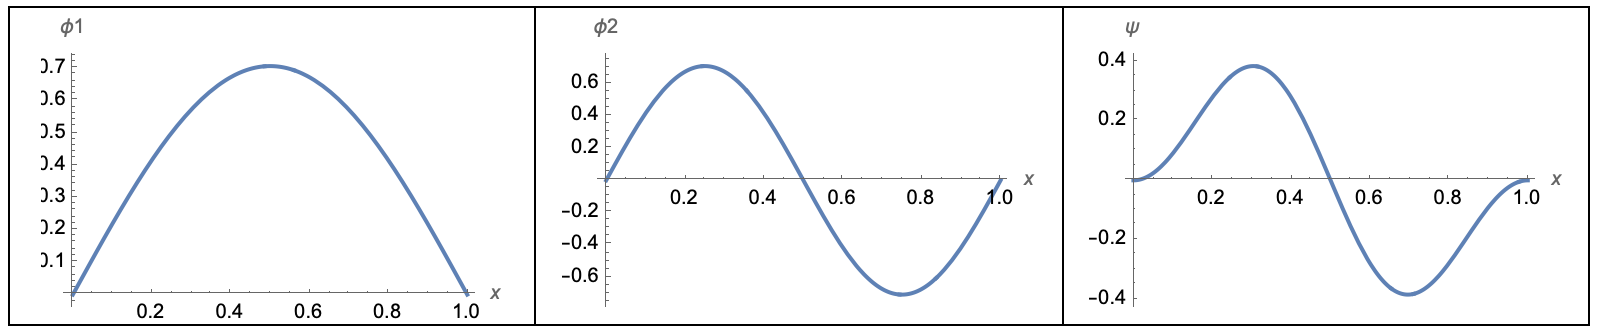
\includegraphics[scale = 0.6]{holestatefunc}	
\centering
\vspace{0.1in}
\caption{Da destra verso sinistra si hanno  le funzioni d'onda $\varphi_1,\varphi_2$ e $\varphi_1\varphi_2$ }
\end{figure}

Nella seguente immagine avremo l'evoluzione temporale del pacchetto di probabilit\`a all'interno della buca infinita di potenziale, procedendo da destra verso sinistra e viceversa. Avremo che in $t = \frac{\pi}{2} \frac{\hbar}{(E_2 - E_1)}$, il coseno in (2.39)  si annulla e la probabilit\`a che la particella si trovi nel centro della buca \`e inferiore a quella che si trovi al lato destro o sinistro della scatola. Come riportato nelle figure centrali. Per $t = \pi \frac{\hbar}{(E_2 -E_1)}$ la probabilit\`a che la particella si trovi al lato sinistro della buca \`e massima.
\begin{figure}[!ht]
\vspace{0.1in}
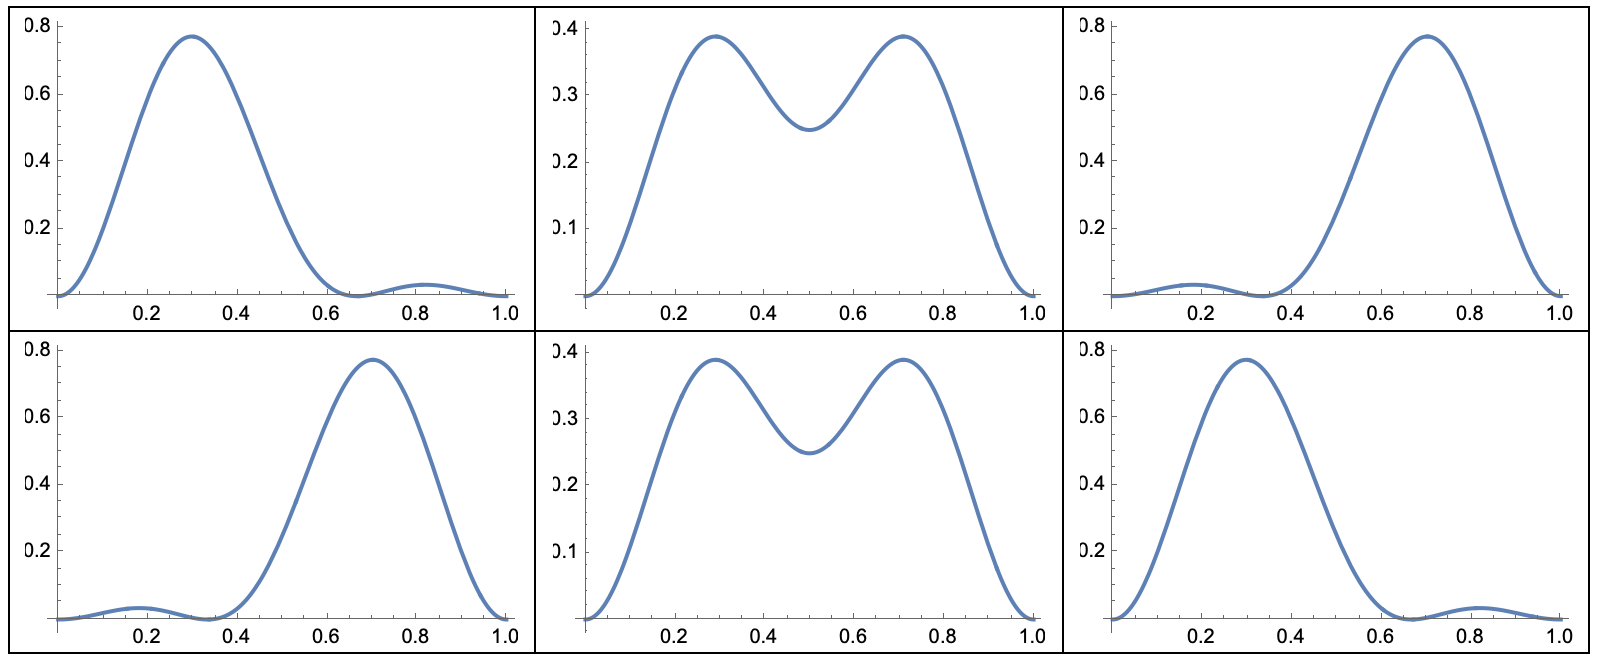
\includegraphics[scale = 0.5]{probevo}	
\centering
\vspace{0.1in}
\end{figure}

In sostanza abbiamo che il pacchetto di probabilit\`a evolve all'interno della buca di potenziale dalle parete infinite, muovendosi avanti e indietro come in figura.

\newpage

\subsection{Esercizio 2: Expanding Box}

Consideriamo una particella confinata in una buca infinita di ampiezza $a$, e nel suo stato fondamentale (\textit{groundstate}), e che istantaneamente si espande raggiungendo un ampiezza $2a$. Determinare la probabilit\`a che la particella resti nello stato fondamentale nel nuovo sistema trasformato.
\begin{figure}[!ht]
\vspace{0.1in}
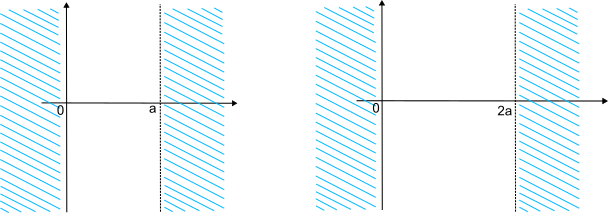
\includegraphics[width = 14cm]{expanding}	
\centering
\end{figure}

Con istantaneamente si intende che la trasformazione avviene cos\`i rapidamente che la particella non ha il tempo di scontare l'informazione, e quindi il suo stato rimane invariato.
\begin{wrapfigure}{l}{0.4\textwidth} % 'r' for right, width of the figure
    \centering
    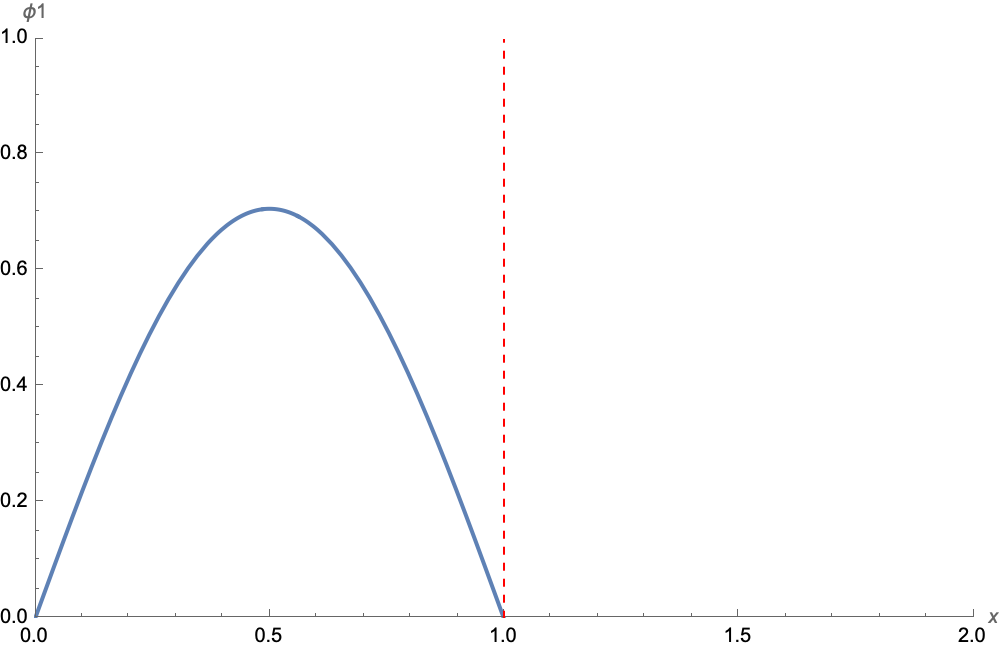
\includegraphics[width=0.4\textwidth]{expstate} % Adjust size and path to image
    \caption{Funzione d'onda allo stato fondamentale per $a=1$.}
\end{wrapfigure}
La funzione d'onda assume l'espressione: 
\begin{equation*}
	\varphi(x) = \left \{ \begin{array}{l}
		 \sqrt{\frac{2}{a}} \sin \left ( \frac{\pi x}{a}\right) \quad 0 <x < a \\[0.5cm]
		 0 \quad a < x <2a
	\end{array}\right.
\end{equation*} 
Raddoppiando la dimensione della buca di potenziale  le autofunzioni della buca iniziale non sono pi\`u le stesse, ma diventano 
\begin{equation*}
	\tilde{\varphi}_n(x) = \sqrt{\frac{2}{2a}}\sin \left (\frac{n\pi x }{2a}\right) = \sqrt{\frac{1}{a}} \sin \left( \frac{n\pi x}{2a}\right) 
\end{equation*}
\newline
I coefficienti delle autofunzioni dello stato iniziale deve essere riscritta rispetto agli elementi della nuova base 
\begin{equation*}
	\varphi(x) = \sum_{n}c_n \tilde{\varphi}_n(x) \quad \text{dove} \quad c_n = \int_0^{2a}dx \; \tilde{\varphi}_n(x) \varphi(x)
\end{equation*}

\begin{figure}[!ht]
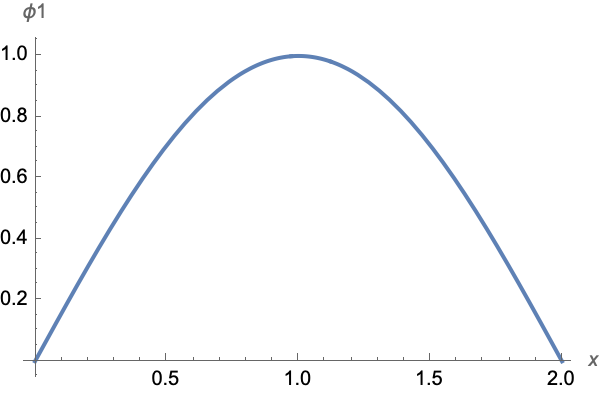
\includegraphics[width = 6cm]{newstate}	
\centering
\caption{Nuovo stato per la buca espansa e a = 2.}
\end{figure}

\newpage 

\begin{proof}
La probabilit\`a che il sistema resti nello stato di partenza \`e data da: 

	\begin{equation*}
		P(\text{fondamentale}) = \left | \int_{0}^{2a}dx \;  \tilde{\varphi_1}(x)\varphi(x) \right |^2 = \left | \int_0^{2a}dx \; \sqrt{\frac{1}{a}}\sin \left(\frac{\pi x}{2a} \right)\sqrt{\frac{2}{a}}\sin \left( \frac{\pi x}{a}\right) \right|^2 = \left| 4\frac{\sqrt{2}}{3\pi}\right|^2
	\end{equation*}
	
\end{proof}
\subsection{Esercizio 3: Rotatore piano}

Consideriamo una particella vincola a muoversi lungo una circonferenza di raggio R. Il moto della particella \`e descritto unicamente dall'angolo $\phi$ e dunque la Hamiltoniana associata \`e data da 
\begin{equation*}
	H = -\frac{\hbar^2}{2I} \frac{d^2}{d\phi^2}
\end{equation*}
dipendendo da un angolo \`e implicito che il problema abbia una sua periodicit\`a $\phi \simeq \phi_0 + 2 \pi$. La trattazione del problemi \`e analoga a quella della buca infinita solo che consideriamo come condizioni al contorno
\begin{equation*}
	\psi(2\pi) = \psi(0) \quad \text{oppure} \quad \psi(\phi+2\pi) = \psi(\phi)
\end{equation*}
che equivale a imporre una certa periodicit\`a nel problema. 

Le autofunzioni e autovalori associati, soluzione dell'equazione di Schr\"odinger
\begin{equation*}
	-\frac{\hbar^2}{2I}\psi_n''(\phi) = E_n\psi(\phi)
\end{equation*}
dove 
\begin{equation*}
	\psi(\phi) = \frac{1}{\sqrt{2\pi}}e^{in\phi} \quad \text{e} \quad E_n = \frac{\hbar^2 n^2}{2I} 
\end{equation*}
Imponendo la condizione di periodicit\`a dobbiamo avere che 
\begin{align*}
	\psi(\phi + 2\pi) = \psi(\phi) \iff & e^{in(\phi + 2\pi)} = e^{in\phi} \\[0.5cm]
	\iff & e^{in 2\pi} = 1 \\[0.5cm]
	\iff & n \in \mathbb{Z}
\end{align*}
Gli stati $\varphi_n(\phi)$ e $ \varphi_{-n}(\phi)$ corrispondono allo stesso livello di energia dato che $E \sim n^2$, l'unica eccezione \`e data da $\varphi_0(\phi)$.
\newline

Utilizzando quanto definito prima, vogliamo determinare l'evoluzione temporale dello stato di partenza dato da 
\begin{equation*}
	\psi(\phi,0) = A \sin^2\phi
\end{equation*}
\newpage

\begin{proof}
	Innanzitutto riscriviamo lo stato iniziale come
	\begin{equation*}
		\psi(0) = A \left( \frac{1-\cos 2\phi}{2} \right) = \frac{A}{2} \left( 1 - \frac{e^{i2\phi} - e^{-i2\phi}}{2}\right)
	\end{equation*} 
riscriviamo lo stato iniziale rispetto alle autofunzioni del rotatore rigido
\begin{equation*}
	\psi(0) = K (2\varphi_0 - \varphi_{2} - \varphi_{-2} )
\end{equation*}
essendo lo spettro della Hamiltoniana discreto, per normalizzare la funzione dobbiamo determinare la costante K, e quindi otteniamo lo stato di partenza 
\begin{equation*}
	\psi(0) = \frac{2\varphi_0 - \varphi_{2} - \varphi_{-2}}{\sqrt{2+1+1}} = \frac{2\varphi_0 - \varphi_{2} - \varphi_{-2}}{\sqrt{6}} 
\end{equation*}
applicando l'operatore di evoluzione temporale $U(t) = e^{- \frac{i}{\hbar}Ht}$ abbiamo che 
\begin{align*}
	\psi(t) = U(t) \psi(0) = & \frac{1}{\sqrt{6}}(2\varphi_0e^{- \frac{i}{\hbar}E_0t} - \varphi_{2}e^{-\frac{i}{\hbar}E_2t} - \varphi_{-2}e^{-\frac{i}{\hbar}E_{-2}t})= \\[0.5cm]
	= & \frac{1}{\sqrt{6}}[2\varphi_0 - e^{-\frac{2 i\hbar^2}{I}t}(\varphi_{2} + \varphi_{-2})] \\[0.5cm]
	= & \frac{1}{\sqrt{3 \pi}}[1 - e^{-\frac{2i \hbar^2}{I}t}\cos(2\phi)]
\end{align*}

\end{proof}

\subsection{Esercizio 4: Buca infinita in 3D}

L'equazione di schr\"odinger per un sistema di dimensione tre \`e data da
\begin{equation*}
	- \frac{\hbar^2}{2m	} \left ( \frac{d^2}{dx^2} + \frac{d^2}{dy^2} + \frac{d^2}{dz^2}\right)\psi(x,y,z) + V(x,y,z)\psi(x,y,z) = E\psi(x,y,z)
\end{equation*}
dove possiamo considerare il caso in cui il potenziale pu\`o essere fattorizzato in tre termini dipendenti dalle singole coordinate
\begin{equation*}
	V(x,y,z) = K(x) + W(y) +T(z)
\end{equation*}
in questo modo l'equazione di Schr\"odinger diventa
\begin{equation*}
	\left (-\frac{\hbar^2}{2m} \frac{d}{dx^2} +K(x)\right)\psi  + \left( -\frac{\hbar^2}{2m} \frac{d^2}{dy^2} +W(y)\right)\psi + \left( -\frac{\hbar^2}{2m}\frac{d^2}{dz^2} +T(z)\right)\psi = (E_x+E_y +E_z)\psi
\end{equation*}
che possiamo vedere come la somma di tre Hamiltoniane rispetto alla singola coordinata
\begin{equation*}
	H = H_x + H_y + H_z
\end{equation*}

questo equivale ad avere un sistema di tre equazioni differenziali ordinarie del secondo ordine
\newpage 
\begin{equation*}
	\left \{ \begin{array}{l}
		H_x \psi_1(x) = E_x \psi_1(x)\\[0.3cm]
		H_y \psi_2(y) = E_y\psi_2(y) \\[0.3cm]
		H_z \psi_3(z) = E_z \psi_3(z)
	\end{array}\right. 
\end{equation*}
dove la soluzione dell'equazione di Schr\"odinger definita inizialmente pu\`o essere scritta come prodotto di tre funzioni rispetto alle singole coordinate
\begin{equation*}
	\psi(x,y,z) = \psi_1(x)\psi_2(y)\psi_3(z) \quad \text{e} \quad E = E_x + E_y + E_z
\end{equation*}
Se prendiamo una buca infinita in tre dimensioni,con larghezza $\bold{a}$, il potenziale associato \`e dato da 
\begin{wrapfigure}{r}{0.4\textwidth} % {r} for right, {0.4\textwidth} for width
    \centering
    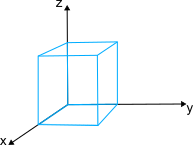
\includegraphics[width=0.38\textwidth]{cube} % Replace with your image
\end{wrapfigure}

\begin{equation*}
	V(x,y,z) = \left \{ \begin{array}{l}
		0 \quad \text{per} \quad x \in [0,a_1]; y\in [0,a_2]; z \in [0,a_3] \\[0.3cm]
		\infty \quad \text{altrimenti}
	\end{array}\right.
\end{equation*}


\noindent Le autofunzioni sono tutti i possibili prodotto della autofunzioni della buca infinita monodimensionale
\begin{align*}
\psi_{n_1}(x) = \sqrt{\frac{2}{a_1} } \sin \left( \frac{n_1 \pi x}{a_1} \right)\\[0.5cm]
\psi_{n_2}(y) = \sqrt{\frac{2}{a_2}} \sin \left ( \frac{n_2\pi y}{a_2}\right) \\[0.5cm]
\psi_{n_3}(z) = \sqrt{\frac{2}{a_3}}\sin \left( \frac{n_3 \pi x}{a_3}\right)
\end{align*}

In notazione di Dirac indichiamo lo stato $|\psi(x,y,z) \rangle = |n_1 \; n_2 \; n_3 \rangle  $. L'auto energia associata \`e espressa come 
\begin{equation*}
	E = \frac{\hbar^2 \pi^2 n_1^2}{2ma_1^2} + \frac{\hbar^2 \pi^2 n_2^2}{2ma_2^2} + \frac{\hbar^2 \pi^2 n_3^2}{2ma_3^2}
\end{equation*}

\subsection{Esercizio 5: Buca infinita in 2D}

Data una particella confinata nel  seguente potenziale 
\begin{equation*}
	V(x,y) = \left \{ \begin{array}{l}
		0 \quad \text{per} \quad x \in [0,a]; y \in [0,a]\\[0.3cm]
		\infty \quad \text{altrimenti}
	\end{array}\right.
\end{equation*}
la cui evoluzione dinamica \`e data dalla Hamiltoniana 
\begin{equation*}
	H = - \frac{\hbar^2}{2m} \left (\frac{d^2}{dx^2} +\frac{d^2}{dy^2}\right) + V(x,y)  
\end{equation*}
\newpage
e che si trova nel seguente stato iniziale 
\begin{equation*}
	\psi = N \cos \left( \frac{\pi x}{a}\right) \cos\left( \frac{\pi y}{a}\right) \sin \left( \frac{2 \pi x}{a}\right)\sin \left( \frac{2 \pi y}{a}\right)
\end{equation*}
determinare: 
\begin{enumerate}
	\item La probabilit\`a rispetto ai livelli di energia dello stato iniziale, il valore di $\langle E \rangle $ e la probabilit\`a per $E_x$.
	\item Se dopo una misurazione si determina che $E_x = \frac{\pi^2 \hbar^2}{2ma^2}$, qual \`e la probabilit\`a che si misuri $E = E_y$ ? 
\end{enumerate}

\begin{proof}
	1) Sappiamo che le autofunzioni soluzione dell'equazione di Schr\"odinger sono 
	\begin{equation*}
		|nm \rangle = \sqrt{\frac{2}{a}} \sin\left(\frac{n\pi x }{a} \right)\sqrt{\frac{2}{a}}\sin \left( \frac{m \pi y}{a}\right)  \quad n,m \in \mathbb{Z}
	\end{equation*}
	e gli autovalori associati sono dati da 
	\begin{equation*}
		E_{nm} = \frac{\hbar^2 \pi^2 n^2}{2\mu a} + \frac{\hbar^2 \pi ^2 m^2}{2 \mu a} \quad n,m \in \mathbb{Z}
	\end{equation*}
Scriviamo lo stato di partenza rispetto alla base formata dalle funzioni $|nm \rangle$
\begin{equation*}
	|\psi\rangle = \frac{|11 \rangle  + |13\rangle + |31\rangle + |33 \rangle }{\sqrt{4}} 
\end{equation*}
le autofunzioni associate sono date dai valori
\begin{equation*}
	E_{11} = \frac{\hbar^2 \pi ^2}{\mu a^2} \quad;\quad  E_{13} = E_{31}=\frac{5\hbar^2 \pi ^2}{\mu a^2}\quad ; \quad E_{33} = \frac{9\hbar^2 \pi^2}{\mu  a^2}
\end{equation*}
La probabilit\`a che la particella si trovi eni diversi stati dell'energia \`e data da 
\begin{equation*}
	P(E=E_{11}) = \frac{1}{4} \quad ; \quad P(E=E{31}=E_{13}) = \frac{1}{4} + \frac{1}{4} = \frac{1}{2} \quad \; \quad P(E=E_{33}) = \frac{1}{4}
\end{equation*}
Il valore medio dell'energia \`e dato da 
\begin{equation*}
	\langle E \rangle = \sum_{n}E_{n}P(E_n) = \frac{1}{4}E_{11} + \frac{1}{2}E_{12} +\frac{1}{4}E_{33} = \frac{5 \hbar^2 \pi^2}{\mu a^2}
\end{equation*}
Infine consideriamo solo i contirbuiti all'energia cinetica rispetto alla coordinata $x$, si ha che 
\begin{align*}
	P \left (E_x = \frac{\hbar^2 \pi^2}{2 \mu a^2}\right ) = \frac{1}{4} + \frac{1}{4} = \frac{1}{2} \\[0.5cm]
	P \left (E_x = \frac{9 \hbar^2 \pi^2}{2\mu a^2}\right )  = \frac{1}{4} + \frac{1}{4} = \frac{1}{2}
\end{align*}
\newpage

2) Dopo aver determinato la probabilit\`a rispetto ad $E_x = \frac{\hbar^2 \pi^2}{2 \mu a^2} $ vogliamo sapere come cambia la probabilit\`a rispetto ad $E_y$.  Dopo aver effettuato una misurazione si ha il collasso della funzione d'onda, dunque la probabilit\`a diventa massima rispetto allo stato osservato, che nel nostro caso \`e dato da 
\begin{equation*}
	|\psi \rangle = \frac{|11 \rangle + |13 \rangle }{\sqrt{2}}
\end{equation*}
La probabilit\`a rispetto ad $y$ assume i seguenti risultati
\begin{align*}
	P \left (E_x = \frac{\hbar^2 \pi^2}{2 \mu a^2}\right ) = ||11\rangle|^2 = \frac{1}{2} \\[0.3cm]
		P \left (E_x = \frac{9 \hbar^2 \pi^2}{2\mu a^2}\right )  = ||13\rangle |^2 = \frac{1}{2}
\end{align*}

\end{proof}

\subsection{Esercizio 6}

Consideriamo un sistema definito su uno spazio di Hilbert $\mathcal{E} = \mathbb{C}^3$, la cui dinamica \`e descritta dalla Hamiltoniana
\begin{equation*}
	H = \hbar \omega_0\left [ \begin{array}{ccc}
		1 & 0 & 0\\
		0 & -1 & 0 \\
		0 & 0 & -1
	\end{array}\right]
\end{equation*} 
dove $\omega_0 \in \mathbb{R}$. Inoltre \`e presente una grandezza fisica osservabile B , il cui operatore associato \`e definito nel seguente modo
\begin{equation*}
	B = b\left [ \begin{array}{ccc}
		1 & 0 & 0\\
		0 & 0 & 1 \\
		0 & 1 & 0
	\end{array}\right]
\end{equation*}
per $b \in \mathbb{R}$. Risolvere i seguenti punti:
\begin{enumerate}
	\item Controllare se $H$ e $B$ sono operatori autoaggiunti.
	\item Determinare una base di autovettori comuni.
	\item Chi tra i seguenti insiemi $\{H\}$,$\{B\}$,$\{B,H\}$ e $\{H^2,B\}$ \`e un sistema di osservabili compatibili completo ? 
\end{enumerate}

\begin{proof}
	1) Una operatore \`e autoaggiunto se $H = H^\dag $ dove $H^\dag = (H^T)^*$, siccome la matrice H \`e diagonale ed \`e costituista da valori reali abbiamo che $H^\dag = H$ e quindi possiamo concludere che la Hamiltoniana del sistema sia un operatore autoaggiunto. Nel caso dell'operatore $\hat{B}$ abbiamo che $B^T = B$ ed \`e anch`esso costituito da valori reali dunque $B^\dag =B$.
	\newline
	
	\noindent 2)Una base comune tra due operatori esiste se e soltanto se questi commutano tra di loro
	\begin{equation*}
		[H,B] = HB -BH = 0
	\end{equation*}
	e quindi l'osservabile B \`e una costante del moto.
	Osserviamo che gli autovettori e autovalori della matrice H sono dati da
	\begin{align*}
	 &\bold{e}_{1} = \left [ \begin{array}{c}
	 	1 \\ 0 \\ 0
	 \end{array}\right] \longrightarrow \lambda_1 = \hbar\omega_0\\[0.5cm]
	  &\bold{e}_{2} = \left [ \begin{array}{c}
	 	0 \\ 1 \\ 0
	 \end{array}\right] \longrightarrow \lambda_2 = -\hbar\omega_0\\[0.5cm]
	  &\bold{e}_{3} = \left [ \begin{array}{c}
	 	0 \\ 0 \\ 1
	 \end{array}\right] \longrightarrow \lambda_3ß = -\hbar\omega_0
	\end{align*}
	Dato che abbiamo degenerazione rispetto agli autovalori, avremo che i vettori che possono essere espressi come
	\begin{equation*}
		\bold{v} = \alpha \bold{e}_2 + \beta \bold{e}_3
	\end{equation*}
	sono autovettori di H con autovalore $\lambda = -\hbar \omega_0$.
	
	Calcoliamo gli autovettori dell'operatore B, osserviamo gi\`a che dalla forma matriciale di tale operatore il vettore $\bold{e}_1$ \`e autovettore di B con autovalore $b$. Per determinare gli altri autovettori calcoliamo le radici associate al polinomio caratteristico della sottomatrice $2 \times 2$ associata a B:
	\begin{equation*}
		P(\lambda) = \text{det} \left [ \begin{array}{cc}
		-\lambda & 1 \\ 1 & -\lambda   
		\end{array} \right ] = \lambda^2-1 = 0
	\end{equation*}
	che ha come radici $\lambda = \pm 1$. Gli autovettori associati sono dati da 
	\begin{align*}
		&\left [ \begin{array}{cc}
		-1 & 1 \\ 1 & -1   
		\end{array} \right ] \left [\begin{array}{c} 
			a \\ b
		\end{array}\right ] = \left [\begin{array}{c} 
			0 \\ 0
		\end{array}\right ] \Rightarrow U_2 = \frac{1}{\sqrt{2}}\left [\begin{array}{c} 
			1 \\ 1
		\end{array}\right ] \rightarrow \lambda =1 \\[0.5cm]
		& \left [ \begin{array}{cc}
		1 & 1 \\ 1 & 1   
		\end{array} \right ] \left [\begin{array}{c} 
			a \\ b
		\end{array}\right ] = \left [\begin{array}{c} 
			0 \\ 0
		\end{array}\right ] \Rightarrow U_3 = \frac{1}{\sqrt{2}}\left [\begin{array}{c} 
			1 \\ -1
		\end{array}\right ] \rightarrow \lambda = -1
	\end{align*}
	che nel caso dell'operatore B hanno autovalore $-b$. Tali autovettori di B sono anche autovettori di H dato che possono essere scritti come combinazione lineare di $\bold{e}_2$ e $\bold{e}_3$. Posto $U_{1} = \bold{e}_{1}$, una base comune ai due operatori \`e data da $\{U_1,U_2,U_3\}$. Dove
	\begin{equation*}
		U_2 = \frac{1}{\sqrt{2}}\left [ \begin{array}{c}
			0 \\ 1 \\ 1
		\end{array}\right] \quad ; \quad U_3 = \frac{1}{\sqrt{2}} \left [ \begin{array}{c}
			0 \\ 1 \\ -1
		\end{array}\right] 
	\end{equation*}
\noindent 3) Compatibile vuol dire che gli operatori presenti nell'insieme commutano tra di loro, mentre con completo si intende che effetuata una misura questa \`e univocamente determinata. Nel nostro caso abbiamo tre vettori $\{U_1,U_2,U_3\}$ e quindi abbiamo tre possibili risultati delle misure.

Consideriamo l'insieme $\{H \}$ e $\{B\}$ tali insiemi sicuramente sono compatibili, ma non completi dato che se effettuiamo una misura e otteniamo come risultato $-\hbar\omega_0$ o $b$, non sappiamo se l'autostato associato \`e dato da $U_2$ o $U_3$ o una loro combinazione lineare, oppure $U_1$ o $U_2$ o una loro combinazione lineare.

L'insieme $\{H^2 ,B \}$ analogamente a quanto discusso prima \`e si formato da operatori completi, ma non compatibili dato che per $b$ o $\hbar^2 \omega_0^2$ si ha degenerazione rispetto agli autostati.

L'ultimo caso da analizzare \`e dato dall'insieme $\{H,B\}$ che risulta essere un sistema completo per quanto verificato al punto 1) e inoltre  \`e completo poich\`e rispetto alla base comuni di autostati $\{U_1,U_2,U_3\}$, abbiamo che le coppie simultanee possibili sono tutte distinte ed associabili a un solo autostato.

\end{proof}

\subsection{Esercizio 7}

Consideriamo un sistema definito su uno spazio di Hilbert $\mathcal{E} = \mathbb{C}^3$, la cui dinamica \`e descritta dalla Hamiltoniana
\begin{equation*}
	H = \hbar \omega_0\left [ \begin{array}{ccc}
		1 & 0 & 0\\
		0 & 2 & 0 \\
		0 & 0 & 2
	\end{array}\right]
\end{equation*} 
dove $\omega_0 \in \mathbb{R}$. Inoltre sono presenti le grandezze fisiche osservabili A e  B , il cui operatore associato \`e definito nel seguente modo
\begin{equation*}
A = a\left [ \begin{array}{ccc}
		1 & 0 & 0\\
		0 & 0 & 1 \\
		0 & 1 & 0
	\end{array}\right] 
	\quad \quad B = b\left [ \begin{array}{ccc}
		0 & 1 & 0\\
		1 & 0 & 0 \\
		0 & 0 & 1
	\end{array}\right] 
\end{equation*}
Inoltre lo stato iniziale del sistema \`e 
\begin{equation*}
	|\psi(0) \rangle = \left[ \begin{array}{c}
		\frac{1}{\sqrt{2}} \\ \frac{1}{2} \\ \frac{1}{2}
	\end{array}\right ]
\end{equation*}
Determinare:
\begin{enumerate}
	\item La probabilit\`a per i livelli di energia E possibili, il valore medio di $\langle E \rangle $, la sua varianza $\Delta E$ al tempo $t=0$.
	\item La probabilit\`a e valori medi per gli osservabili A e B al tempo generico $t$.
\end{enumerate}

\begin{proof}
	1) Gli autovalori associati alla Hamiltoniana sono dati dagli elementi della base canonica $\{\bold{e}_{1},\bold{e}_{2},\bold{e}_3\}$ con i corrispettivi autovalori $\{\hbar \omega_0,2\hbar \omega_0,2\hbar \omega_0 \}$. Riscriviamo lo stato inzile rispetto a tale base 
	\begin{equation*}
		|\psi(0) \rangle = \frac{1}{\sqrt{2}}\bold{e}_1 + \frac{1}{2} \bold{e}_2 + \frac{1}{2} \bold{e}_{3}
	\end{equation*}
Calcoliamo la probabilit\`a che il sistema si trovi negli stati energetici definiti dalla 
Hamiltoniana
\begin{equation*}
P(E = \hbar\omega_0) = \left | \frac{1}{\sqrt{2}} \right |^2 = \frac{1}{2} \quad ; \quad P(E = 2 \hbar \omega_0) = \frac{1}{4} + \frac{1}{4} = \frac{1}{2} 	
\end{equation*}
Il valore medio dell'energia \`e dato da
\begin{equation*}
	\langle E \rangle = \sum_{n} E_n P(E=E_n) = \hbar \omega_0 \frac{1}{2} + 2 \hbar \omega_0 \frac{1}{2} = \frac{3}{2}\hbar \omega_0
\end{equation*}
la deviazione standard associata viene calcolata nel seguente modo
\begin{equation*}
	\Delta E = \sqrt{\langle E^2 \rangle - \langle E \rangle ^2} 
\end{equation*}
calcoliamo il termine
\begin{equation*}
	\langle E^2 \rangle = \sum_{n}E_n^2 P(E_n) = \hbar^2 \omega_0^2 \frac{1}{2}  + \frac{1}{2}4 \hbar^2 \omega_0^2 = \frac{5}{2}\hbar^2 \omega_0^2
\end{equation*}
quindi l'incertezza sulla misura dell'energia \`e data da 
\begin{equation*}
	\Delta E = \sqrt{\frac{5}{2} \hbar^2 \omega_0^2 - \frac{9}{4} \hbar^2 \omega_0^2} = \frac{1}{2}\hbar \omega_0
\end{equation*}
2) Per determinare l'evoluzione temporale dello stato applichiamo l'operatore di evoluzione temporale allo stato iniziale $|\psi(0) \rangle $, ovvero
\begin{equation*}
	|\psi \rangle = U(t)|\psi(0) \rangle = e^{- \frac{i}{\hbar}Ht}|\psi(0)\rangle 
\end{equation*}
ottenendo
\begin{equation*}
	|\psi(t) \rangle = \frac{1}{\sqrt{2}} e^{-i\omega_0 t}\bold{e}_{1}+ \frac{1}{2} e^{-2i\omega_0t}\bold{e}_{2} + \frac{1}{2}e^{-2i \omega_0 t}\bold{e}_{3}
\end{equation*}
Procediamo con il calcolare gli autovettori e autovalori dell'operatore $\hat{A}$. Determinando
\begin{equation*}
	U_1 = \bold{e}_{1} \rightarrow \lambda = a \quad ; \quad U_2 = \frac{1}{\sqrt{2}}\left [ \begin{array}{c}
			0 \\ 1 \\ 1
		\end{array}\right]  \rightarrow \lambda = a \quad ; \quad U_3 = \frac{1}{\sqrt{2}}\left [ \begin{array}{c}
			0 \\ 1 \\ -1 
		\end{array}\right]\rightarrow \lambda = -a 
\end{equation*}

La probabilit\`a associata alle due misure possibili dell'osservabile $A$ \`e data da 
\begin{equation*}
	P(A = -a) = |\langle U_3 | \psi(t) \rangle |^2 = \left |\frac{1}{\sqrt{2}} [0 \; 1 \; -1]^* \cdot \left [ \begin{array}{c}
		\frac{e^{-i \omega_0t}}{\sqrt{2}} \\ \frac{e^{-i2 \omega_0 t}}{2} \\ \frac{e^{-i2 \omega_0 t}}{2}
	\end{array}\right] \right|^2 = 0
\end{equation*}	
dato che la somma delle probabilit\`a degli stati deve essere uguale a uno, possiamo concludere che $P(A = a) =\frac{1}{2} + \frac{1}{2} = 1$.
Infinite calcoliamo il valore medio di A
\newpage

\begin{equation*}
	\langle A \rangle = \sum_{n}AP(A) = aP(A=a)-aP(A =-a) =a
\end{equation*}
in alternativa possiamo procedere al calcolo considerando
\begin{equation*}
	\langle \psi(t)|A|\psi(t) \rangle = \left [ \frac{e^{-i \omega_0t}}{\sqrt{2}} \\ \frac{e^{-i2 \omega_0 t}}{2} \\ \frac{e^{-i2 \omega_0 t}}{2}\right] a \left [ \begin{array}{ccc}
		1 & 0 & 0\\
		0 & 0 & 1 \\
		0 & 1 & 0
	\end{array}\right] \left [ \begin{array}{c}
		\frac{e^{-i \omega_0t}}{\sqrt{2}} \\ \frac{e^{-i2 \omega_0 t}}{2} \\ \frac{e^{-i2 \omega_0 t}}{2}
	\end{array}\right] = a
\end{equation*}
Analoga discussione viene fatta per le grandezza richieste relative all'osservabile B.

\end{proof}

\subsection{Esercizio 8: Notazione di Heisenberg}

Consideriamo una particella soggetta al potenziale $V(x) = - fx$. Qual \`e il valore di $\Delta p(t) ?$

\begin{proof}
	Per rispondere alla domanda usiamo la notazione di Heisenberg rispetto a cui vale la relazione 
	\begin{equation*}
		\frac{d}{dt}A_H = \frac{\partial A_H}{\partial t} + \frac{1}{i \hbar}[A_H,H]
	\end{equation*}
	dove definiamo $A_H$, ovvero la rappresentazione di un generico operatore A nella notazione di Heinsenberg, nel seguente modo
	\begin{equation*}
		\langle A \rangle = \langle \psi(t) |A|\psi(t) \rangle = \langle \psi(t_0)|e^{\frac{i}{\hbar}H(t-t_0)}Ae^{\frac{i}{\hbar}H(t-t_0)}|\psi(0)\rangle   = \langle \psi(0)|A_H|\psi(0) \rangle 
	\end{equation*}
e quindi 
\begin{equation*}
	A_H = e^{\frac{i}{\hbar}H(t-t_0)}Ae^{\frac{i}{\hbar}H(t-t_0)}
\end{equation*}
Utilizzando tale notazione gli operatori momento e posizione definiscono il seguente sistema di equazioni
\begin{equation*}
	\left \{ \begin{array}{l}
		\frac{d}{dt}x_H = \frac{p_H}{m} \\[0.3cm]
	  \frac{d p_H}{dt} = -V'(x_H) = f
	\end{array}\right.
\end{equation*}	
ottenendo la seguente legge orarie
\begin{equation*}
x_H = \frac{f}{2m}t^2 + \frac{p_0}{m}t +x_0
\end{equation*}
che abbiamo ottenuto calcolando
\begin{equation*}
	p_H(t) = ft + p_0
\end{equation*}
e sostituendolo nella quadratura della prima equazione. Utilizzando tale risultato intermedio procediamo a calcolare l'incertezza sui momenti, dove
\begin{equation*}
	\langle p_h \rangle  = \langle \psi(0) | p_h |\psi(0) \rangle = ft + \langle p_0\rangle = \langle p \rangle  
\end{equation*} 
\newpage 


si ha che l'uguaglianza coincide con quella nella notazione di Dirac. Da qui in poi si procede come negli esercizi precedenti, calcolando il risultato intermedio
\begin{equation*}
	\langle p^2 \rangle = \langle (ft+p_0)^2 \rangle = f^2t^2 + 2ft \langle p_0 \rangle + \langle p_0 \rangle^2
\end{equation*}
Infine 
\begin{equation*}
	\Delta p^2 = \langle p^2 \rangle - \langle p \rangle ^2 = f^2t^2 + 2ft \langle p_0 \rangle + \langle p_0^2\rangle - f^2t^2-2ft\langle p_0 \rangle - \langle p_0 \rangle^2 = \langle p_0^2 \rangle - \langle p_0 \rangle^2 = \Delta p^2(t=0) 
\end{equation*}
La varianza dell'operatore p resta costante nel tempo.
\end{proof}
